\section{Results}
\label{sec:results}

\paragraph{Results convention.}
All numerical results below are contract-scoped diagnostics. A row is treated as paper-facing evidence only when its emitted convergence and validation-status fields say so; otherwise it remains a diagnostic artifact for model development rather than a benchmark claim. This convention replaces repeated per-paragraph disclaimers.


The results are organized around the analyses supporting claims C1--C5. First, forward renders and composite-particle examples show one shared scene represented across multiple configured microscopes. Second, Cram\'{e}r--Rao orderings, fusion diagnostics, and Fisher density maps evaluate the information layer per microscope. Third, deterministic supervision-schema evaluations check that measurement support, ignore masks, and loss-weight outputs follow the declared policy. The configured-profile comparison tables in this section use one shared instrument configuration and vary only the contrast modality; they are therefore the fixed-instrument special case of the general cross-microscope comparison defined in \cref{subsec:microscope-unit}, and each row should be read as a microscope whose instrument parameters happen to be held in common.

\subsection{Forward-model demonstrations}

\paragraph{Modality panel.} The same latent particle state is rendered through the forward-modality panel. The aligned panels in \cref{fig:modality-panel} present one particle/sample state under different contrast mechanisms; the shared scene and display field, rather than a separate single-modality simulation, are held fixed across panels, and each panel records its resolved sampling in the generated manifest.

\IfFileExists{figures/imaging-modes.png}{%
\begin{figure}[H]
\centering
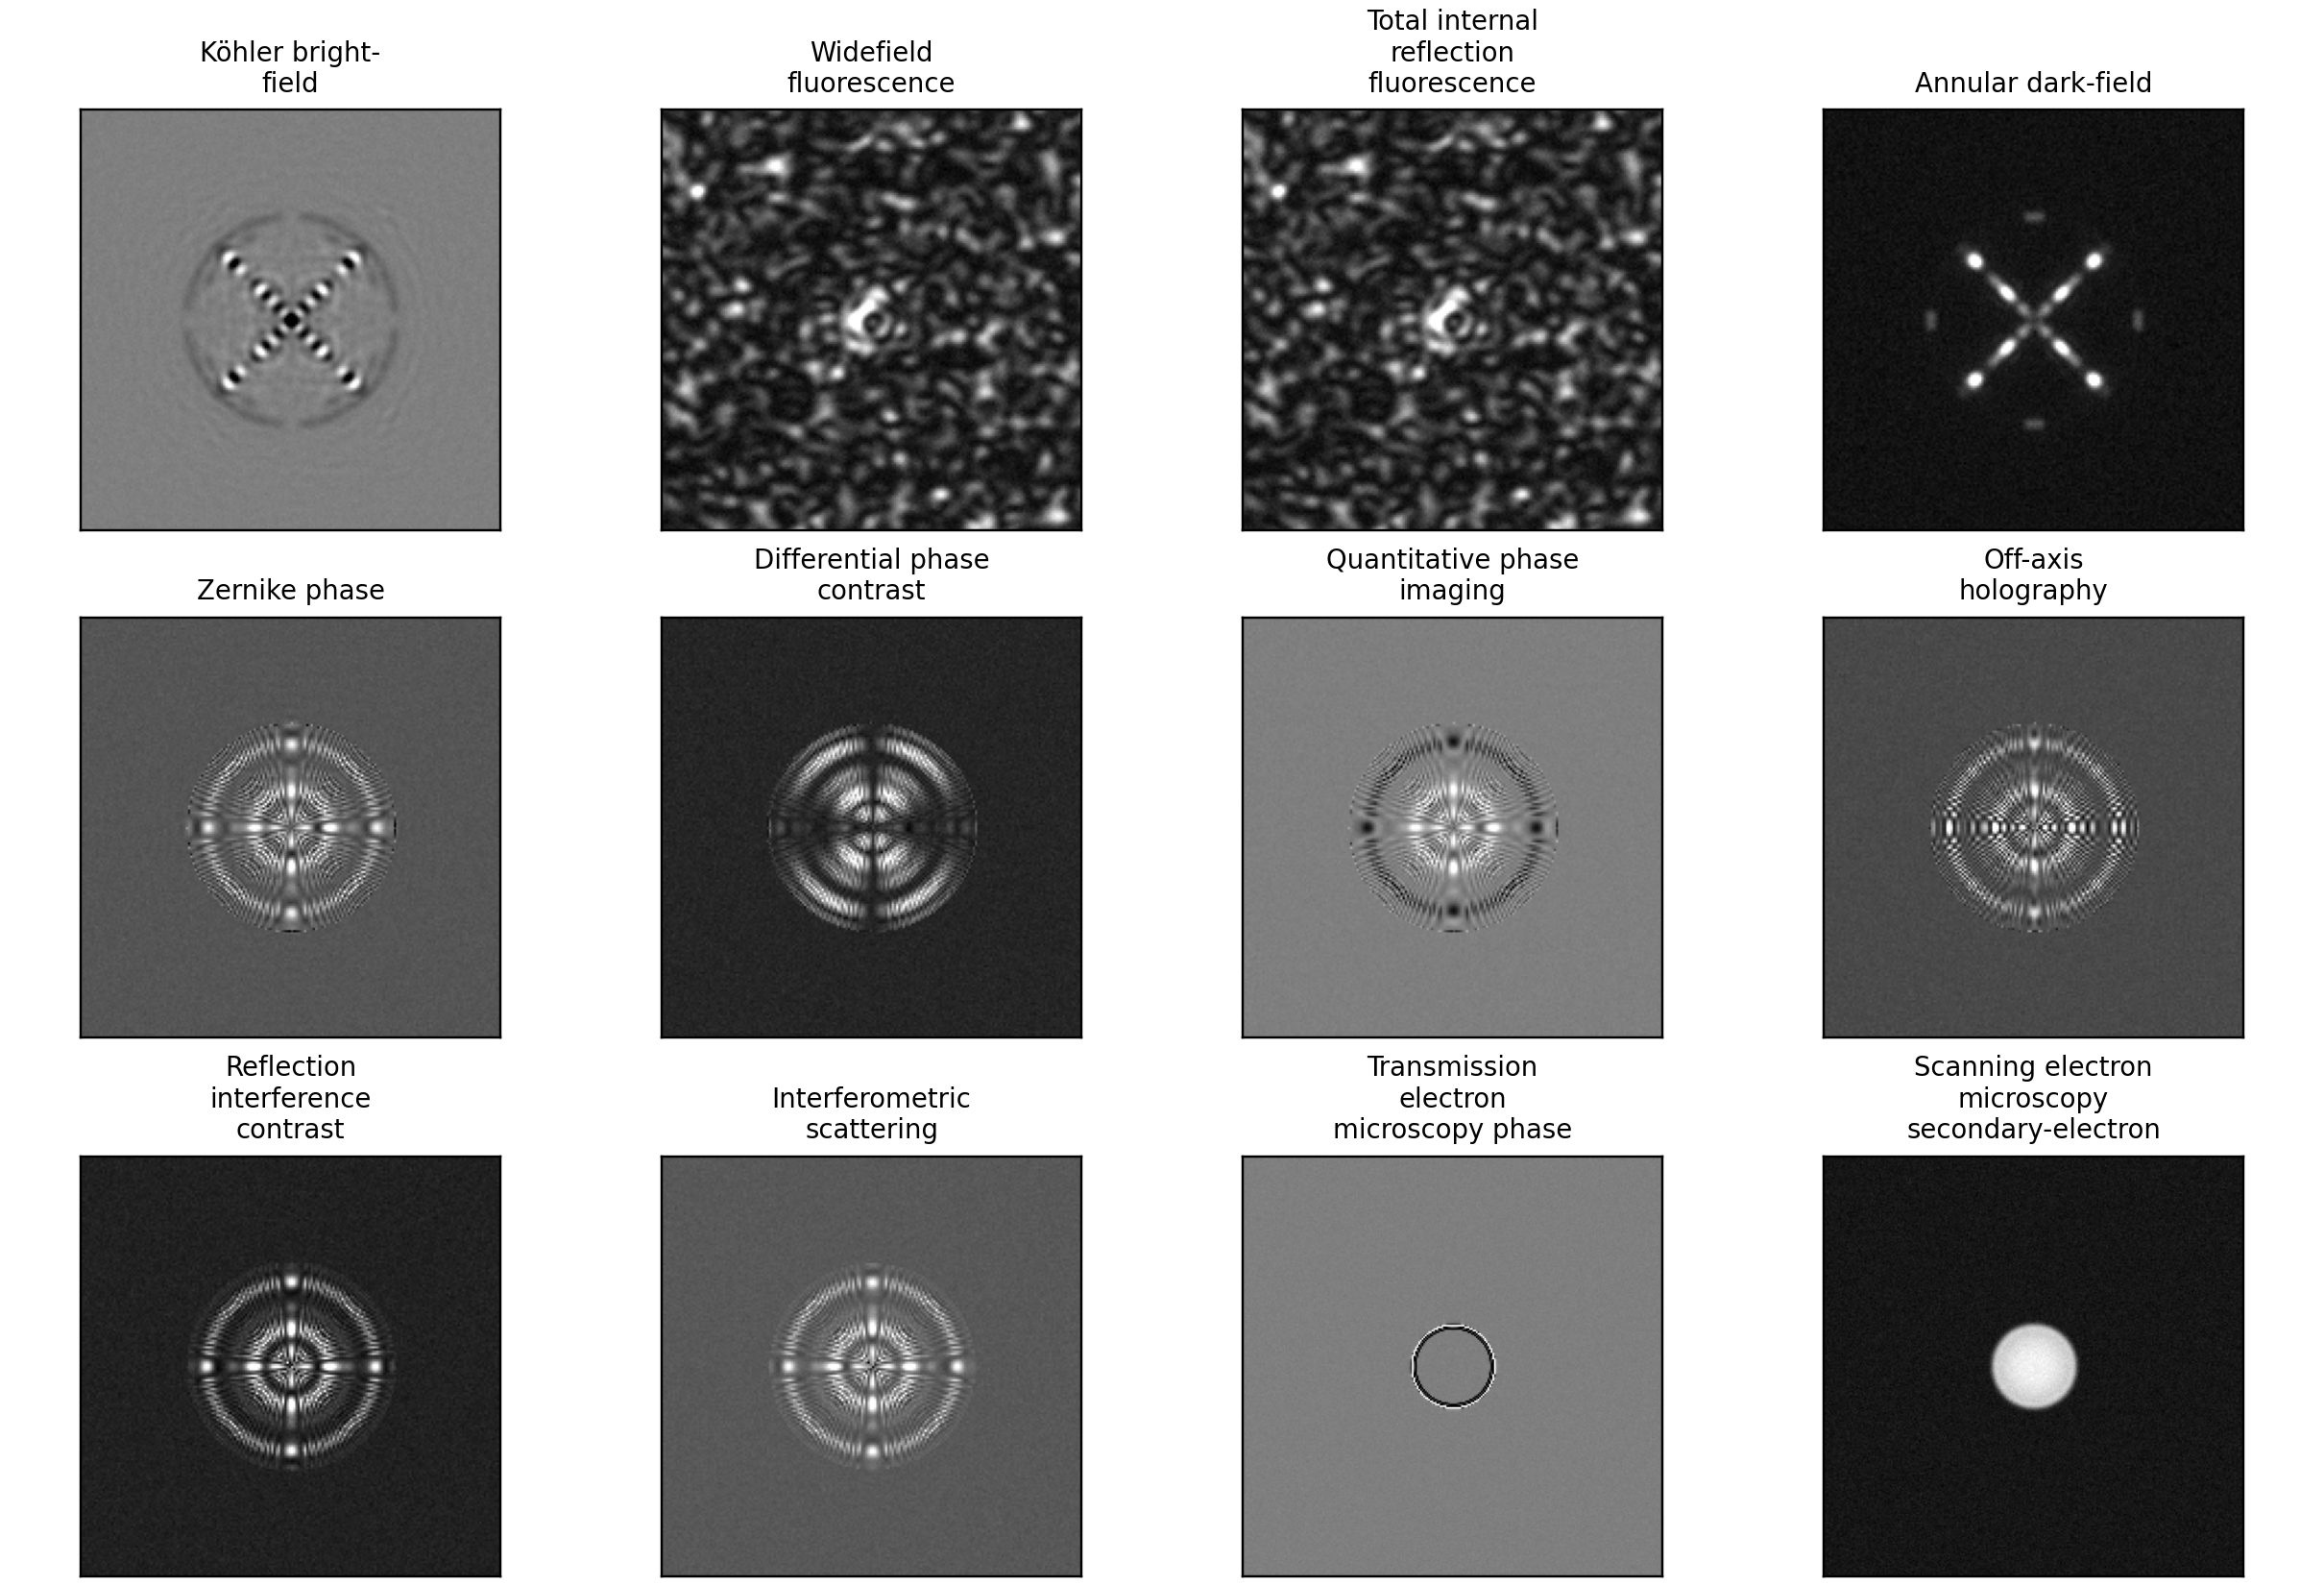
\includegraphics[width=\linewidth]{figures/imaging-modes.png}
\caption{Modality panel. The same latent particle state is rendered through the forward-modality panel on a common physical display field. Each panel is a camera-style windowed detector or phase display with an embedded scale bar; signed-contrast diagnostic arrays and resolved sampling metadata are saved separately for quantitative inspection.}
\label{fig:modality-panel}
\end{figure}
}{%
\generatedfallbackfigure{fig:modality-panel}{Modality panel. The same latent particle state is rendered through the forward-modality panel on a common physical display field.}{Required figure asset.}
}

\paragraph{Composite-particle rendering.} Composite particles are represented as rigid assemblies of primitive components --- spheres and non-spherical primitives such as ellipsoids and rods --- with body-frame offsets. The panel in \cref{fig:composite-gallery} shows representative rendered frames for a sphere, an ellipsoid, a rod (cylinder primitive), a dimer, a linear trimer, a bent triatomic, a bowtie-like assembly, and a tetrahedral 3D assembly under matched camera, imaging-model, and noise settings. The gallery includes non-spherical primitives so the rendered geometry is not restricted to isotropic spheres; compact assemblies can still project similarly, so orientation identifiability is quantified separately for the $\mathrm{SE}(3)$ diagnostic subset in \cref{tab:orientation-crlb}.

\IfFileExists{figures/composite-gallery.png}{%
\begin{figure}[H]
\centering
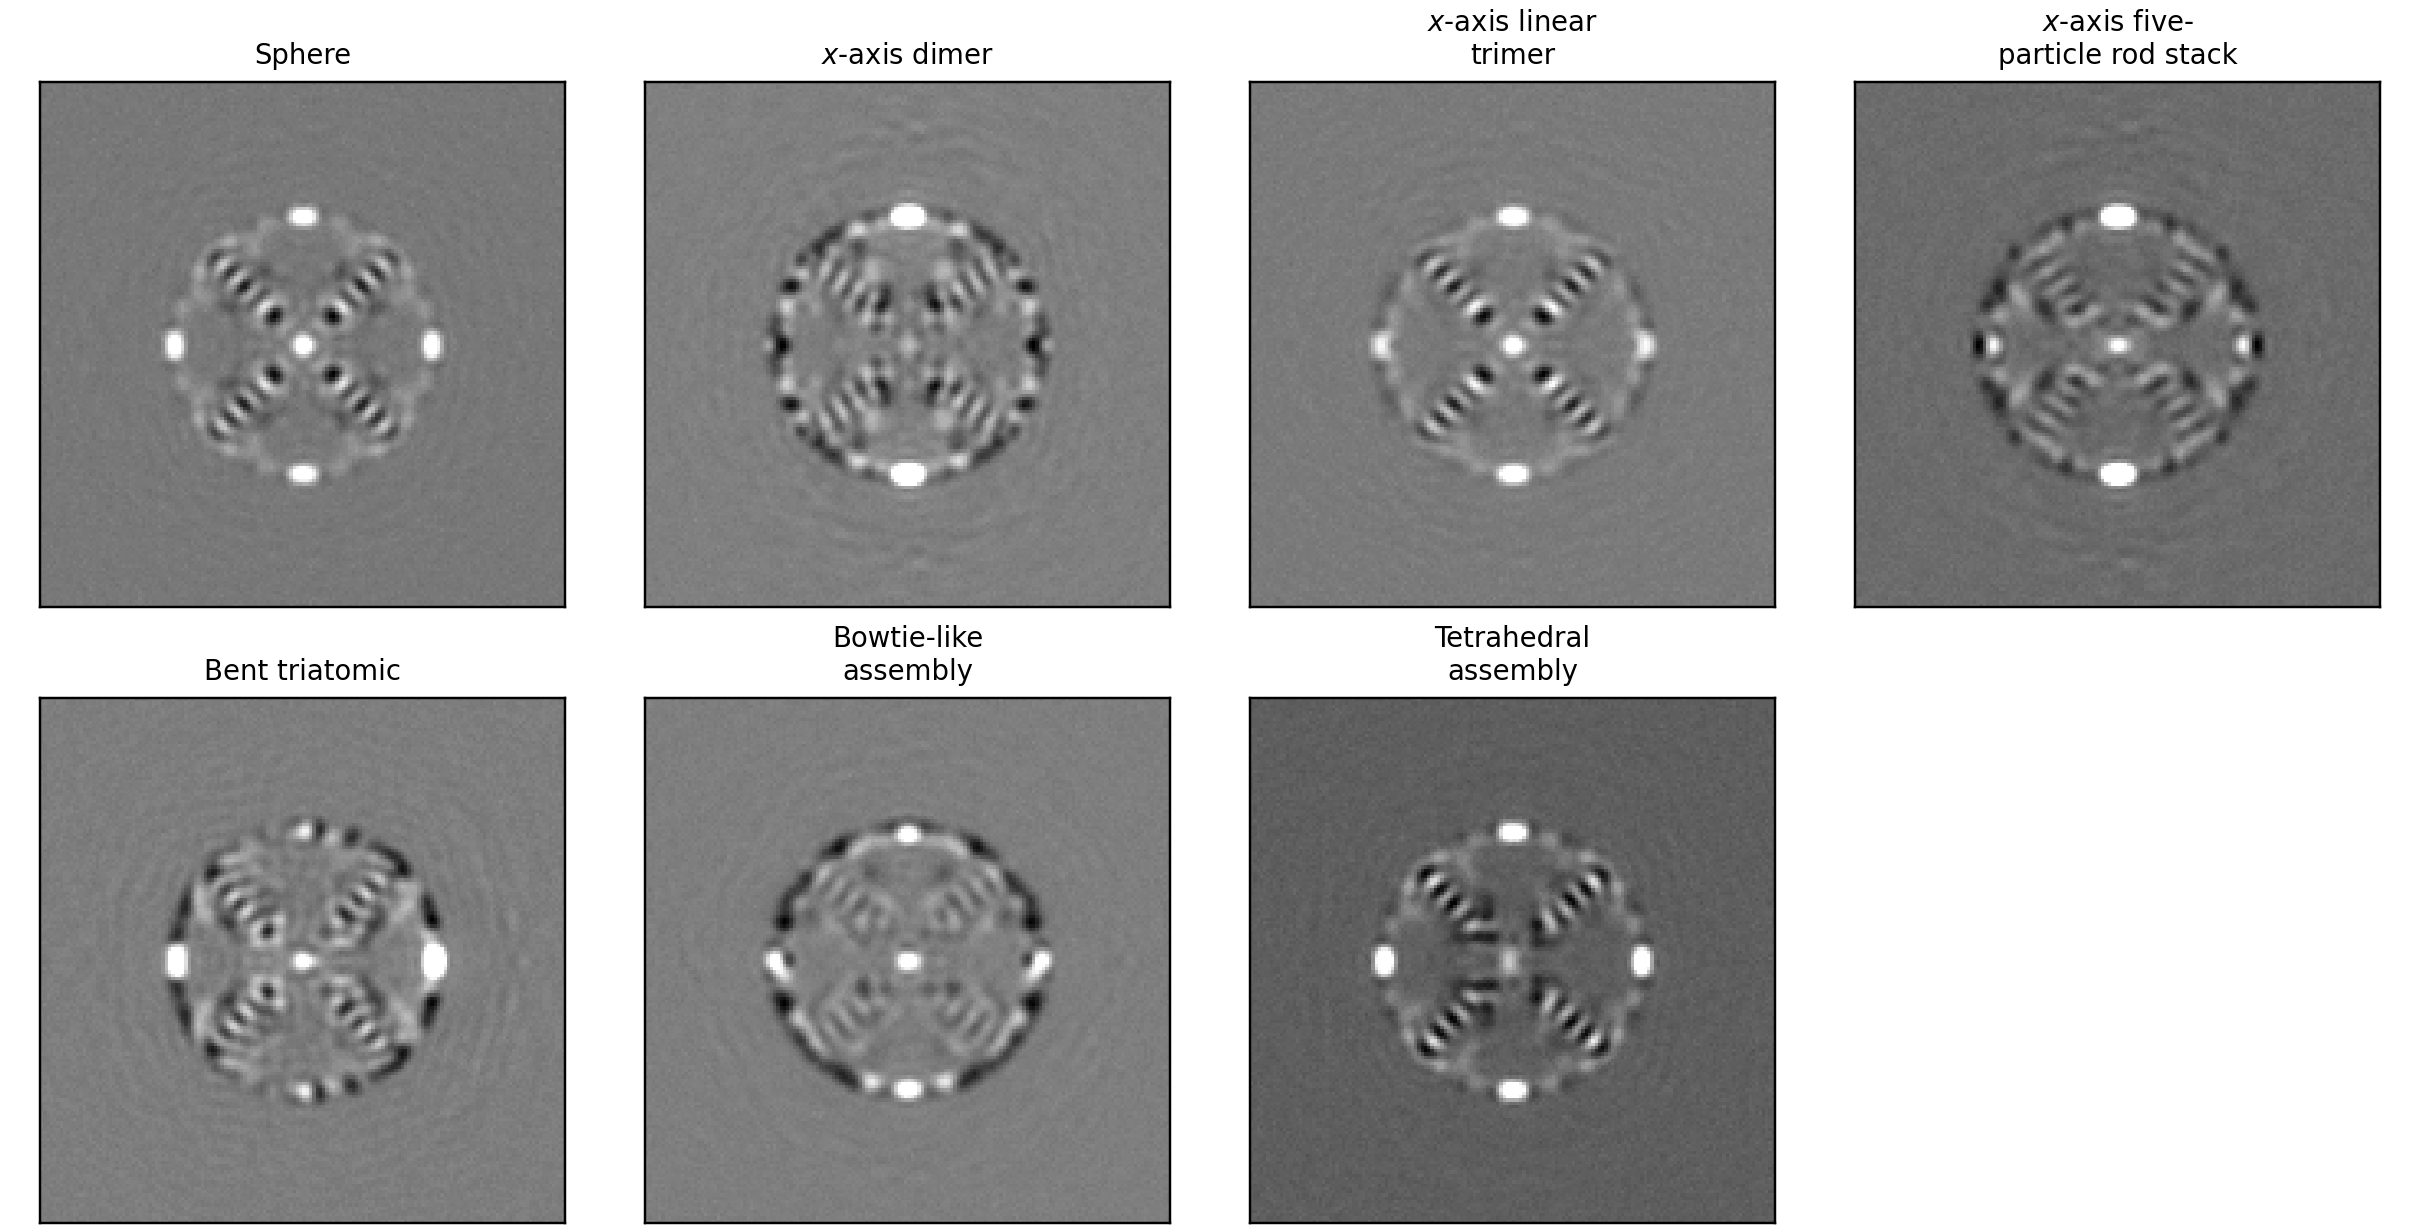
\includegraphics[width=\linewidth]{figures/composite-gallery.png}
\caption{Composite particle gallery. The displayed shapes are rendered under identical camera, imaging-model, and noise settings. Compact assemblies can project similarly in this display; \cref{tab:orientation-crlb} reports orientation-rank diagnostics for the subset used in the $\mathrm{SE}(3)$ check.}
\label{fig:composite-gallery}
\end{figure}
}{%
\generatedfallbackfigure{fig:composite-gallery}{Composite particle gallery. The displayed shapes are rendered under identical camera, imaging-model, and noise settings.}{Required figure asset.}
}

\paragraph{Coupled-cluster scattering.} For closely spaced components the independent-superposition model is not the right physical object, so Syniscopy partitions a particle's components into interaction clusters by exact inter-component surface gap and solves close clusters with a coupled solver (Section~\ref{sec:physical-model}). \Cref{tab:coupled-scattering-demo} demonstrates this on a dimer whose inter-component gap is swept: at large gap the coupled solver reproduces the independent superposition (the decoupling limit), and as the gap closes the coupled contrast and lateral Cram\'{e}r--Rao bound diverge from the superposition while the coupling-regime gate marks the uncoupled proxy invalid. This both validates the coupled solver against the decoupling limit and shows the regime where the uncoupled model would misstate the bound.

\IfFileExists{figures/coupled-scattering-demo-table.tex}{%
\begin{table}[H]
\centering
\small
\resizebox{\linewidth}{!}{\input{figures/coupled-scattering-demo-table}}
\caption{Coupled-cluster scattering demonstration on a dimer at decreasing inter-component surface gap. The coupled solver's contrast and lateral Cram\'{e}r--Rao bound are compared against the independent (uncoupled) superposition, alongside the cluster-partition coupling-regime gate. Large gaps recover the superposition (decoupling limit); small gaps diverge and the gate flags the uncoupled proxy as invalid.}
\label{tab:coupled-scattering-demo}
\end{table}
}{%
\generatedfallbacktable{tab:coupled-scattering-demo}{Coupled-cluster scattering demonstration: coupled vs uncoupled dimer contrast and Cram\'{e}r--Rao bound across inter-component gap, with the coupling-regime gate.}{Required table asset.}
}

\subsection{Cram\'{e}r--Rao and Fisher information diagnostics}

\paragraph{Theory-to-diagnostic map.}
Each formal statement in \cref{sec:information-layer} is paired with a simulator diagnostic in \cref{tab:theoretical-support}. The table lists, for each theorem, corollary, or operational diagnostic, the output used to inspect the corresponding behavior.

\IfFileExists{figures/theoretical-support-table.tex}{%
\begin{table}[H]
\centering
\small
\resizebox{\linewidth}{!}{\begin{tabular}{@{}>{\raggedright\arraybackslash}p{0.18\linewidth}>{\raggedright\arraybackslash}p{0.28\linewidth}>{\raggedright\arraybackslash}p{0.28\linewidth}>{\raggedright\arraybackslash}p{0.18\linewidth}@{}}
\toprule
Claim & What it says & Simulator diagnostic & Output shown in \\
\midrule
Symmetry rank theorem & Contrast-functional continuous symmetry predicts $\mathrm{SE}(3)$ rank deficit. & Rank predictor plus observed Fisher rank and singular-axis metadata. & Table~\ref{tab:orientation-crlb}. \\
Fusion-symmetry corollary & Fusion breaks only rotation symmetries not shared by each selected modality. & Fused-rank predictor from the intersection stabilizer dimension. & Tables~\ref{tab:orientation-crlb} and~\ref{tab:fusion-symmetry-diagnostic}. \\
Reject-rule support-score decomposition & Supported supervision uses bounded signal, information, temporal, and ambiguity support factors combined as clipped log odds by default. & Supervision consistency evaluation for representative supported, borderline, and excluded targets. & Table~\ref{tab:supervision-audit}. \\
Registration covariance & Registration uncertainty monotonically weakens fused information. & Registration-adjusted bound and degradation fraction. & Table~\ref{tab:registration-degradation}. \\
Loewner dominance & Loewner-dominated information-rate matrices can be pruned for fixed-budget scheduling. & Synthetic two-matrix dominance check and Loewner-maximal set. & Table~\ref{tab:loewner-dominance}. \\
Structured-background nuisance projection & Structured background removes the nuisance-subspace projection of signed particle derivatives. & Raw and nuisance-adjusted Fisher summaries for a synthetic background basis. & Table~\ref{tab:structured-background-loss}. \\
Detected-quanta scaling & Poisson-dominated detected-quanta scaling changes the Cram\'{e}r--Rao bound as $1/\sqrt{\alpha}$ when normalized image shape and detector regime are fixed. & Fixed-budget ordering and detected-quanta sweep. & Table~\ref{tab:budget-normalized}; Fig.~\ref{fig:detected-quanta-budget-pareto}. \\
Diminishing fusion returns & Best-$k$ fusion bounds can saturate under a supplied modality set. & Best-$k$ fusion curve under the implemented modality set. & Fig.~\ref{fig:fusion-curve}. \\
\bottomrule
\end{tabular}
}
\caption{How the theoretical contributions map to simulator diagnostics. Established mathematical tools are used where stated; the paper's contributions are the shared-scene Fisher information framing, the contrast-symmetry rank theorem and fusion corollary, the matched microscope-packet format, and the reject-rule support-score supervision decomposition as implemented diagnostics.}
\label{tab:theoretical-support}
\end{table}
}{%
\generatedfallbacktable{tab:theoretical-support}{How the theoretical contributions map to simulator diagnostics.}{Required table asset.}
}

\begin{table}[H]
\centering
\small
\begin{tabular}{p{0.26\linewidth}p{0.64\linewidth}}
\toprule
Parameter & Diagnostic profile value \\
\midrule
Particle & 100~nm gold sphere unless varied; the same particle material state is passed to every microscope, while each microscope's contrast modality supplies its own response and noise parameters \\
Image grid & Head-to-head modality contracts use a shared \(192\times192\) detector grid, 65~nm pixel pitch, 384 pupil samples, and \(2\times\) point-spread-function oversampling; native-regime source-use rows are separate source-specific cases \\
Optical medium/objective & water medium $n=1.33$; immersion $n=1.518$; profile-specific numerical aperture or probe scale \\
Wavelength & 532~nm profile unless a modality profile overrides it (vectorial Debye default; scalar paraxial selectable) \\
Derivative and singularity rules & lateral spectral band-limited derivatives with Nyquist/boundary diagnostics; axial planes at $z_0\pm200$~nm; $\mathrm{SE}(3)$ orientation perturbations of 0.03~rad; singular axes use a scale-relative Fisher eigenvalue tolerance of $10^{-12}$ \\
Noise and budget & propagated detector noise for configured-profile rankings; $N_Q=5\times10^4$ for budget-normalized Poisson/phase diagnostics \\
\bottomrule
\end{tabular}
\caption{Representative diagnostic profile conventions for the configured-profile Cram\'{e}r--Rao examples in this section. These values are not a calibration of any specific bench; absolute bounds depend on supplied amplitude, detector, shared sampling, and noise parameters.}
\label{tab:default-profile}
\end{table}

\paragraph{Closed-form scaling checks.} The lateral Cram\'{e}r--Rao implementation includes checks against three expected laws: $\sigma_{xy}\propto 1/\mathrm{SNR}$ at fixed point-spread-function width, $\sigma_{xy}\propto d^{-3}$ for a controlled Rayleigh-amplitude response, and diameter-independence at fixed signal-to-noise ratio \cite{thompson-larson-webb,ober-ram-ward,juffmann-iscat-cobri-crlb}. \Cref{tab:closed-form-scaling-checks} reports the fitted exponent or residual for each check. These are software consistency diagnostics under controlled inputs, not empirical validation of microscope performance. The Rayleigh row holds the image geometry and noise fixed while scaling contrast amplitude as $d^3$, so the Fisher bound should scale as $d^{-3}$. The fixed-SNR diameter-independence check is a renormalized control in which the signal amplitude is held fixed as diameter changes; both controls are separate from the particle-size sweep in \cref{fig:particle-size-sweep}, where modality-specific contrast amplitude and noise can vary with diameter while the head-to-head observation grid is held fixed.

\IfFileExists{figures/closed-form-scaling-check-table.tex}{%
\begin{table}[H]
\centering
\small
\resizebox{\linewidth}{!}{\begin{tabular}{p{0.22\linewidth}p{0.34\linewidth}rrp{0.22\linewidth}}
\toprule
Check & Input sweep/control & Expected exponent & Fitted exponent & Residual summary \\
\midrule
Detected-quanta/SNR scaling & native interfero\allowbreak{}metric scattering microscopy SNR proxy sqrt(N\_Q) sweep & $-1.000$ & -1.000 & 1.000000; max rel. residual 0.0013\% \\
Rayleigh interfero\allowbreak{}metric scattering microscopy diameter scaling & controlled Rayleigh-amplitude Fisher sweep & $-3.000$ & -3.000 & 1.0000; max rel. residual 0.00\% \\
Fixed-SNR diameter control & diameter label varied with contrast/noise arrays held fixed & $0.000$ & 0.000 & max rel. change 0.000\% \\
\bottomrule
\end{tabular}
}
\caption{Closed-form scaling checks for the Fisher implementation. The first row uses the native iSCAT detected-quanta sweep converted to the Poisson-limited signal-to-noise proxy $\sqrt{N_Q}$, the Rayleigh row uses a controlled fixed-geometry contrast-amplitude sweep, and the fixed-SNR row is the renormalized control in which contrast and noise arrays are held fixed.}
\label{tab:closed-form-scaling-checks}
\end{table}
}{}

\paragraph{Configured-profile lateral Cram\'{e}r--Rao diagnostic.} Microscopes are reported under the shared instrument configuration summarized in \cref{tab:default-profile}; generated profile-card artifacts, when present, provide the per-microscope backend-fidelity cards. This head-to-head diagnostic is the fixed-instrument special case: it holds detector sampling and optics fixed across the compared microscopes and lets the contrast modality, backend, material/source interpretation, and detector-noise/count settings define the comparison. A general cross-microscope comparison instead lets each microscope carry its own optics and detector configuration; \Cref{tab:cross-microscope-comparison} reports such a comparison, in which microscopes that share a contrast modality but differ in instrument configuration (for example numerical aperture, pixel pitch, or detected-quanta budget) receive distinct Cram\'{e}r--Rao bounds. That two same-modality microscopes are ranked separately, rather than collapsed into one modality row, is the property that makes the microscope --- not the bare modality --- the unit of comparison. The lateral derivative implementation is checked in \cref{tab:lateral-spectral-diagnostics}: the bound uses the single center-rendered contrast image and the exact spectral gradient, while the table reports whether the sampled image is sufficiently band-limited and contained in the field of view.

\IfFileExists{figures/cross-microscope-comparison-table.tex}{%
\begin{table}[H]
\centering
\small
\resizebox{\linewidth}{!}{\input{figures/cross-microscope-comparison-table}}
\caption{Cross-microscope comparison in which candidates that share a contrast modality differ in instrument configuration. Each row is a microscope; rows with the same modality but different numerical aperture, pixel pitch, or detected-quanta budget report distinct lateral Cram\'{e}r--Rao bounds, so they are ranked as separate candidates rather than merged into one modality entry. This is the general case for which the configured-profile table in \cref{tab:modality-ranking} is the fixed-instrument special case.}
\label{tab:cross-microscope-comparison}
\end{table}
}{%
\generatedfallbacktable{tab:cross-microscope-comparison}{Cross-microscope comparison: same-modality microscopes with differing instrument configuration receive distinct Cram\'{e}r--Rao bounds and are ranked as separate candidates.}{Required table asset.}
}

\paragraph{Comparison contracts.} Table-to-table claims are contract-specific in this section. We use four explicit contracts: Contract-LP (configured-profile lateral Cram\'{e}r--Rao), Contract-LZ (configured-profile axial/\(\mathrm{SE}(3)\) diagnostics), Contract-Q (detected-quanta-normalized comparison), and Contract-NR (native-regime source-use context). The same profile can therefore produce different orderings under different contracts.

Cram\'{e}r--Rao lower bounds in \Cref{tab:modality-ranking} are Contract-LP diagnostics over microscopes that share one instrument configuration: each row is a microscope reported on a shared physical coordinate frame with shared detector pitch and its own contrast-modality response/noise backend, not a native-instrument comparison. Because the instrument is held fixed, the table doubles as the fixed-instrument modality comparison. Bench mapping is approximate: the current configuration parameters do not absorb all stray light, alignment error, out-of-focus particles, dust, or detector nonlinearity; source-matching residuals are addressed explicitly through configurable sample-environment perturbations including \texttt{sample\_environment\_pattern\_roughness\_model}, \texttt{sample\_environment\_pattern\_roughness\_amplitude}, \texttt{sample\_environment\_pattern\_roughness\_correlation\_pixels}, \texttt{sample\_environment\_pattern\_roughness\_phase\_std}, and \texttt{sample\_environment\_pattern\_roughness\_source} (for \texttt{source\_matched} mode), with roughness-source coupling options \texttt{independent}, \texttt{coherent\_amplitude}, \texttt{field\_weighted}, \texttt{scene\_weighted}, and \texttt{channel\_weighted} (default: \texttt{channel\_weighted}). The transmission-electron-microscopy row uses its configured backend-specific dose and potential/contrast settings \texttt{ctf\_proxy}/\texttt{multislice\_lite}/\texttt{syniscopy\_multislice}; native transmission-electron-microscopy sampling remains a separate instrument-specific configuration in Contract-NR.

\Cref{tab:modality-ranking} reports the default Contract-LP configured-profile diagnostic bound and within-profile relative bound. Table~\ref{tab:lateral-spectral-diagnostics} reports the sampling and support diagnostics attached to the same lateral Fisher calculation, so Table~\ref{tab:modality-ranking} should be read as a status-tagged configured-profile diagnostic rather than a universal ranking independent of sampling and field containment. Under the spectral lateral calculation, the lowest lateral bounds are scanning electron microscopy secondary-electron, interferometric scattering microscopy, and off-axis digital holography in this configured profile; rows with large Nyquist-band energy or boundary energy should not be used for precise numerical claims without rerunning at an adequate field size and detector sampling. The differential-phase-contrast row is reported via the configured vectorial Debye asymmetric-illumination model: opposite half-disc condenser-source images are rendered, passed through shifted objective pupils, differenced, and normalized. Metadata records the selected DPC transfer model, illumination sigma, source sampling count, channel model, and vectorial detection mode; split-pupil/Foucault and phase-gradient proxy DPC are explicit alternate settings rather than the default row.

\IfFileExists{figures/modality-profile-card-table.tex}{%
\begin{table}[H]
\centering
\small
\resizebox{\linewidth}{!}{\begin{tabular}{p{0.18\linewidth}p{0.18\linewidth}p{0.17\linewidth}p{0.18\linewidth}p{0.15\linewidth}p{0.14\linewidth}}
\toprule
Modality & Profile/fidelity & Domain/units & Paper category & Validation & Scope \\
\midrule
partially coherent Köhler bright-field & vectorial\_abbe\_kohler\_bright\_field & contrast/relative\_reference & core\_scalar\_optical\_profile & unchecked & model-conditioned shared-scene diagnostic under the listed profile parameters \\
widefield fluorescence & vectorial\_photophysics\_fidelity\_based & count/detector\_count & core\_scalar\_optical\_profile & diagnostic only & model-conditioned shared-scene diagnostic under the listed profile parameters \\
total internal reflection fluorescence & vectorial\_photophysics\_fidelity\_based & count/detector\_count & core\_scalar\_optical\_profile & diagnostic only & model-conditioned shared-scene diagnostic under the listed profile parameters \\
annular Köhler dark-field & scalar\_abbe\_annular\_kohler\_dark\_field & count/detector\_count & core\_scalar\_optical\_profile & unchecked & model-conditioned shared-scene diagnostic under the listed profile parameters \\
Zernike phase contrast & model\_conditional\_profile & count/detector\_count & scalar\_proxy\_profile & unchecked & model-conditioned shared-scene diagnostic under the listed profile parameters \\
differential phase contrast & model\_conditional\_profile & count/detector\_count & scalar\_proxy\_profile & unchecked & model-conditioned shared-scene diagnostic under the listed profile parameters \\
quantitative phase imaging & model\_conditional\_profile & phase/radian & phase\_domain\_profile & unchecked & model-conditioned shared-scene diagnostic under the listed profile parameters \\
off-axis digital holography & model\_conditional\_profile & fringe\_count/detector\_count & scalar\_proxy\_profile & unchecked & model-conditioned shared-scene diagnostic under the listed profile parameters \\
reflection interference contrast microscopy & model\_conditional\_profile & contrast/relative\_reference & scalar\_proxy\_profile & unchecked & model-conditioned shared-scene diagnostic under the listed profile parameters \\
interfero\allowbreak{}metric scattering microscopy & model\_conditional\_profile & contrast/relative\_reference & core\_scalar\_optical\_profile & unchecked & model-conditioned shared-scene diagnostic under the listed profile parameters \\
transmission electron microscopy phase contrast & syniscopy\_multislice\_physics\_based & electron\_count/electron\_count & high\_fidelity\_electron\_profile & diagnostic only & model-conditioned shared-scene diagnostic under the listed profile parameters \\
scanning electron microscopy secondary-electron & syniscopy\_transport\_sem\_lite & electron\_count/electron\_count & high\_fidelity\_electron\_profile & diagnostic only & model-conditioned shared-scene diagnostic under the listed profile parameters \\
\bottomrule
\end{tabular}
}
\caption{Human-readable modality profile cards used by the configured-profile tables. Full machine-readable profile identifiers are retained in the generated artifact manifest and supplemental metadata.}
\label{tab:modality-profile-cards}
\end{table}
}{}

Total internal reflection fluorescence and widefield fluorescence are separate configured fluorescence profiles in \cref{tab:modality-ranking}. A separate native-regime source-use audit row for total internal reflection fluorescence exercises angle-derived evanescent excitation and trajectory depth; that audit row is not the configured-profile ranking row in \cref{tab:modality-ranking}.

Appendix~\ref{sec:source-use-audit} reports the native-regime source-use audit. That audit documents source use, source category, parameter-match status, computed localization scale where applicable, and source-reported scale. Only source categories that report or derive a localization scale populate the computed-localization column; dimensional-metrology and modality-principle rows are retained for provenance without being treated as particle-center localization checks. In particular, the native interferometric-scattering audit path uses the opt-in Fresnel-reference and high-numerical-aperture dipole-collection controls and gives a nanometer-scale result under that native check, whereas the configured-profile interferometric-scattering row belongs to the cross-modality diagnostic table.

The annular K\"{o}hler dark-field row is finite under the configured gold-particle scattering profile. Singular entries, when they occur, indicate that the selected diagnostic image provides no finite Fisher bound under that profile, not that experimental dark-field localization is impossible.

\IfFileExists{figures/modality-ranking-table.tex}{%
\begin{table}[H]
\centering
\small
\resizebox{\linewidth}{!}{\begin{tabular}{r p{0.26\linewidth} p{0.22\linewidth} r r p{0.16\linewidth}}
\toprule
Order & Modality & Profile/fidelity & $\sigma_{xy}$ (nm) & Relative $\sigma_{xy}$ & Status \\
\midrule
1 & Zernike phase contrast & model\_conditional\_profile & 0.013 & 1.000 & failed convergence \\
2 & interfero\allowbreak{}metric scattering microscopy & model\_conditional\_profile & 0.017 & 1.271 & failed convergence \\
3 & off-axis digital holography & model\_conditional\_profile & 0.042 & 3.209 & failed convergence \\
4 & scanning electron microscopy secondary-electron & syniscopy\_transport\_sem\_lite & 0.043 & 3.237 & failed convergence \\
5 & differential phase contrast & model\_conditional\_profile & 0.098 & 7.470 & failed convergence \\
6 & reflection interference contrast microscopy & model\_conditional\_profile & 0.150 & 11.41 & failed convergence \\
7 & quantitative phase imaging & model\_conditional\_profile & 1.290 & 98.08 & failed convergence \\
8 & transmission electron microscopy phase contrast & syniscopy\_multislice\_physics\_based & 1.879 & 142.9 & failed convergence \\
9 & partially coherent Köhler bright-field & vectorial\_abbe\_kohler\_bright\_field & 40.55 & 3084.1 & failed convergence \\
10 & annular Köhler dark-field & scalar\_abbe\_annular\_kohler\_dark\_field & 586.1 & 44576.6 & failed convergence \\
11 & total internal reflection fluorescence & vectorial\_photophysics\_fidelity\_based & 96359.5 & 7.329e+06 & failed convergence \\
12 & widefield fluorescence & vectorial\_photophysics\_fidelity\_based & 96398.0 & 7.331e+06 & failed convergence \\
\bottomrule
\end{tabular}
}
\caption{Default Contract-LP lateral Cram\'{e}r--Rao diagnostic values using the spectral band-limited lateral derivative. The table reports Syniscopy diagnostic values only and should not be read as a native-instrument benchmark independent of the sampling/support status; native-regime literature scale checks are separated into the source-use audit in Appendix~\ref{sec:source-use-audit}.}
\label{tab:modality-ranking}
\end{table}
}{%
\generatedfallbacktable{tab:modality-ranking}{Configured-profile lateral Cram\'{e}r--Rao ordering over the configured modality profiles.}{Required table asset.}
}

Lateral rows are no longer accepted or rejected by a finite-difference step sweep, because the lateral derivative has no perturbation step. Instead, \Cref{tab:lateral-spectral-diagnostics} reports the physical sampling/support diagnostics that determine whether the spectral derivative is trustworthy for the configured grid.

\IfFileExists{figures/lateral-spectral-diagnostics-table.tex}{%
\begin{table}[H]
\centering
\small
\resizebox{\linewidth}{!}{\input{figures/lateral-spectral-diagnostics-table}}
\caption{Lateral spectral-derivative sampling diagnostics for the configured-profile Cram\'{e}r--Rao diagnostic. The lateral Fisher matrix is computed from the exact FFT gradient of the center-rendered contrast image; the diagnostic columns report the derivative basis, Nyquist-band energy fraction, boundary energy fraction, numerical rank, and row status used to decide whether the sampled image is adequately band-limited and field-contained.}
\label{tab:lateral-spectral-diagnostics}
\end{table}
}{%
\generatedfallbacktable{tab:lateral-spectral-diagnostics}{Lateral spectral-derivative sampling diagnostics for the configured-profile Cram\'{e}r--Rao diagnostic.}{Required table asset.}
}

\paragraph{Partial-order comparison.} The scalar bound in \Cref{tab:modality-ranking} is one projection of the comparison, not the verdict. Because the central claim is that there is no universal ordering, the comparison is reported as a partial order. \Cref{tab:partial-order-comparison} gives two views over the same candidate set. The Loewner information order marks a candidate as information-dominated when another candidate's Fisher matrix is at least as large on every parameter direction ($F_A-F_B\succeq 0$); this is contract-independent and compares the information itself rather than a scalarization. The multi-criterion Pareto front is taken over localization precision together with the supplied acquisition-cost axes (dose, acquisition time, and a destructiveness flag); a candidate is dominated only when another is no worse on every axis and strictly better on at least one. Two candidates can therefore be genuinely incomparable --- one more precise, the other lower-dose or non-destructive --- and the front is the set of defensible choices rather than a single winner. The scalar rank is shown only as a reference projection.

\IfFileExists{figures/partial-order-comparison-table.tex}{%
\begin{table}[H]
\centering
\small
\resizebox{\linewidth}{!}{\input{figures/partial-order-comparison-table}}
\caption{Partial-order microscope comparison over the configured candidate set. Columns report whether each candidate is Loewner-information-maximal, whether it lies on the multi-criterion Pareto front over precision and the supplied acquisition-cost axes, the candidate(s) that dominate it when it is off the front, and its scalar rank as a reference projection. Candidates on the front are mutually incomparable defensible choices; a single scalar ranking would hide that.}
\label{tab:partial-order-comparison}
\end{table}
}{%
\generatedfallbacktable{tab:partial-order-comparison}{Partial-order microscope comparison: Loewner-information-maximal set and multi-criterion Pareto front over precision and acquisition-cost axes, with the scalar rank as a reference projection.}{Required table asset.}
}

\Cref{fig:particle-size-sweep} shows the corresponding particle-size sweep. Diameter-dependent contrast scaling can change the ordering, so the sweep should not be read as a universal modality ranking for every contract or as the fixed-SNR diameter-independence check above.

\IfFileExists{figures/particle-size-sweep.png}{%
\begin{figure}[H]
\centering
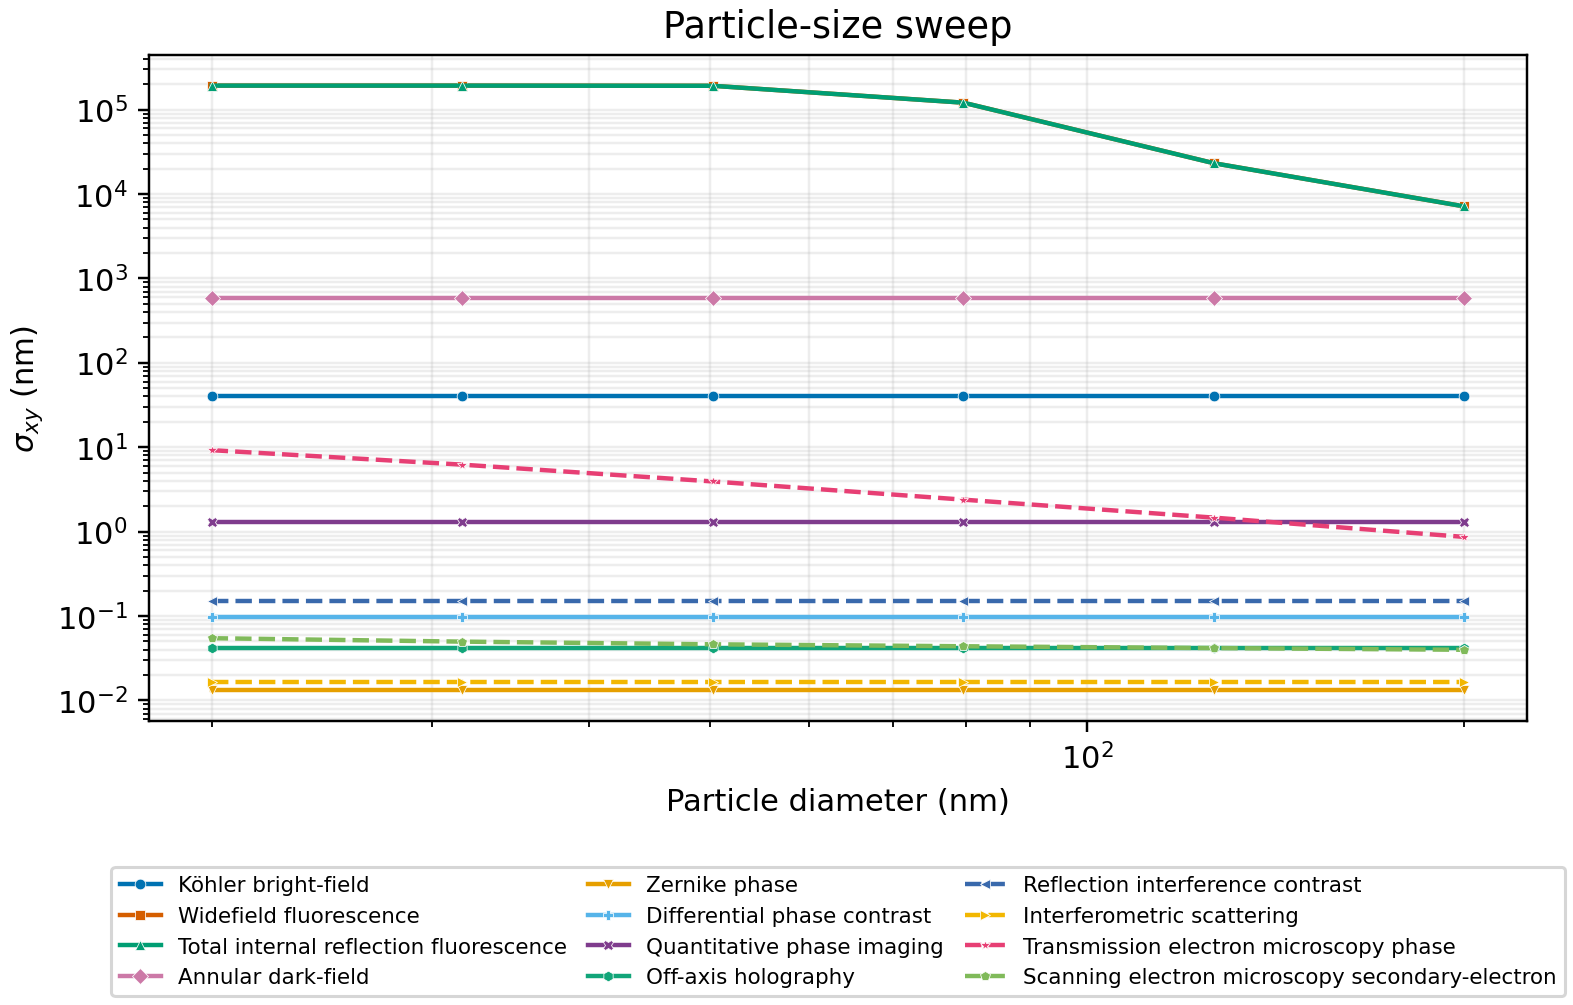
\includegraphics[width=0.85\linewidth]{figures/particle-size-sweep.png}
\caption{Particle-size sweep under the Contract-LP spectral lateral-derivative convention. Each color/marker/line-style combination is one imaging modality, identified by the legend below the axes. The curves expose how diameter-dependent contrast scaling can change modality diagnostics across particle sizes. Unless separately regenerated with per-diameter spectral sampling/support metadata, these curves inherit the configured-grid assumptions in Table~\ref{tab:lateral-spectral-diagnostics}; singular cases are treated as nonfinite rather than assigned artificial finite values.}
\label{fig:particle-size-sweep}
\end{figure}
}{%
\generatedfallbackfigure{fig:particle-size-sweep}{Particle-size sweep. The curves expose how diameter-dependent contrast scaling can change fixed-instrument candidate diagnostics across particle sizes. Singular cases are treated as nonfinite rather than assigned artificial finite values.}{Required figure asset.}
}

\paragraph{Axial and orientation bounds.} Contract-LZ uses a three-plane axial extension at $z_0-\Delta z$, $z_0$, and $z_0+\Delta z$, and reports default $\sigma_z$ values and singular rows in \cref{tab:axial-crlb}. The $\mathrm{SE}(3)$ extension uses one center render plus symmetric perturbation pairs for $z$, $\omega_x$, $\omega_y$, and $\omega_z$, where $\omega$ denotes an infinitesimal body-frame rotation. Symmetric composites report singular body axes explicitly in \cref{tab:orientation-crlb}. The diagnostic subset includes anisotropic primitives (a true rod and an ellipsoid) and a coupled cluster, so the reported continuous symmetries arise from intrinsic particle anisotropy rather than from the isotropy of spherical sub-components. Most finite axial rows in \Cref{tab:axial-crlb} fail the axial derivative-step convergence gate (Table~\ref{tab:axial-convergence-crlb}); widefield fluorescence, TEM phase contrast, and SEM remain singular under this Contract-LZ setup. Therefore this table is an axial singularity/diagnostic report, not a universal claim of native axial instrument performance.

\IfFileExists{figures/orientation-crlb-table.tex}{%
\begin{table}[H]
\centering
\small
\resizebox{\linewidth}{!}{\begin{tabular}{lcccccc}
\toprule
Particle & Numerical Fisher rank & Axis-estimability rank & Stabilizer $d$ & Null rotation axes $\ge d$ & Generic rank & Singular rotation axes \\
\midrule
Sphere & 3 & 3 & 3 & 3 & 3 & rotation about $x$, rotation about $y$, rotation about $z$ \\
$x$-axis dimer & 5 & 5 & 1 & 1 & 5 & bond-axis rotation \\
$x$-axis linear trimer & 5 & 5 & 1 & 1 & 5 & chain-axis rotation \\
Bent triatomic & 6 & 6 & 0 & 0 & 6 & none \\
$x$-axis five-particle rod stack & 5 & 5 & 1 & 1 & 5 & rod-axis rotation \\
Tetrahedral assembly & 6 & 6 & 0 & 0 & 6 & none \\
\bottomrule
\end{tabular}
}
\caption{$\mathrm{SE}(3)$ rank and singular-axis metadata by composite shape. The numerical Fisher rank is shown beside the axis-estimability rank, the rank predicted from continuous contrast symmetry, and the guaranteed number of null rotation axes; $\omega_x,\omega_y,\omega_z$ are infinitesimal body-frame rotations about the principal axes.}
\label{tab:orientation-crlb}
\end{table}
}{%
\generatedfallbacktable{tab:orientation-crlb}{$\mathrm{SE}(3)$ rank and singular-axis metadata by composite shape. The numerical Fisher rank and axis-estimability rank are shown beside the symmetry-predicted generic rank and the symmetry-guaranteed nullity lower bound.}{Required table asset.}
}

\IfFileExists{figures/orientation-spectrum-table.tex}{%
\begin{table}[H]
\centering
\small
\resizebox{\linewidth}{!}{\begin{tabular}{p{0.24\linewidth}rrrp{0.32\linewidth}}
\toprule
Particle & Numerical rank & Rank tol. & Cond. & Fisher eigenvalues \\
\midrule
Sphere & 3 & 2.213e-19 & 11.34 & 0.000000e+00;0.000000e+00;0.000000e+00;1.950746e-08;2.200424e-07;2.213089e-07 \\
$x$-axis dimer & 5 & 2.739e-12 & 9.605e+07 & -1.424544e-23;2.851051e-08;2.748695e-07;3.920763e-07;7.154251e-03;2.738545e+00 \\
$x$-axis linear trimer & 5 & 3.032e-12 & 2.207e+07 & -2.581085e-21;1.373882e-07;1.191681e-06;1.758532e-06;2.435891e-02;3.032129e+00 \\
Bent triatomic & 6 & 2.710e-12 & 1.915e+08 & 1.414638e-08;3.082185e-07;4.799763e-07;1.412055e-02;2.222073e-02;2.709711e+00 \\
$x$-axis five-particle rod stack & 5 & 6.759e-12 & 5.332e+07 & 5.870607e-22;1.267657e-07;6.826466e-07;1.706997e-06;1.061646e-01;6.758892e+00 \\
Tetrahedral assembly & 6 & 3.895e-12 & 8.709e+07 & 4.471888e-08;4.213445e-07;4.598425e-07;6.979435e-01;3.880060e+00;3.894585e+00 \\
\bottomrule
\end{tabular}
}
\caption{$\mathrm{SE}(3)$ Fisher spectrum metadata for the orientation-rank diagnostic. The table records the eigenvalue spectrum and rank tolerance used to declare singular axes.}
\label{tab:orientation-spectrum}
\end{table}
}{}

\IfFileExists{figures/orientation-rank-convergence-table.tex}{%
\begin{table}[H]
\centering
\small
\resizebox{\linewidth}{!}{\begin{tabular}{p{0.30\linewidth}p{0.23\linewidth}p{0.23\linewidth}c}
\toprule
Particle & Numerical ranks over $\delta\omega$ & Singular axes over $\delta\omega$ & Pass \\
\midrule
Sphere & 0.015:3; 0.030:3; 0.060:3 & 0.015:omega\_x, rotation about $y$, rotation about $z$, 0.030:omega\_x, rotation about $y$, rotation about $z$, 0.060:omega\_x, rotation about $y$, rotation about $z$ & yes \\
$x$-axis dimer & 0.015:5; 0.030:5; 0.060:5 & 0.015:omega\_x, 0.030:omega\_x, 0.060:omega\_x & yes \\
$x$-axis linear trimer & 0.015:5; 0.030:5; 0.060:5 & 0.015:omega\_x, 0.030:omega\_x, 0.060:omega\_x & yes \\
Bent triatomic & 0.015:6; 0.030:6; 0.060:6 & 0.015:none, 0.030:none, 0.060:none & yes \\
$x$-axis five-particle rod stack & 0.015:5; 0.030:5; 0.060:5 & 0.015:omega\_x, 0.030:omega\_x, 0.060:omega\_x & yes \\
Tetrahedral assembly & 0.015:6; 0.030:6; 0.060:6 & 0.015:none, 0.030:none, 0.060:none & yes \\
\bottomrule
\end{tabular}
}
\caption{$\mathrm{SE}(3)$ orientation-step convergence check. The numerical Fisher rank and singular-axis labels are recomputed across symmetric body-frame rotation perturbations and must remain stable for the diagnostic to pass.}
\label{tab:orientation-rank-convergence}
\end{table}
}{}

\Cref{tab:fusion-symmetry-diagnostic} records the cross-modality fusion-symmetry case on a single fixed particle geometry, separately from the per-shape table. The two fused entries are two modalities imaging the \emph{same} particle: one modality's contrast functional retains a continuous rotational symmetry that the other modality's contrast functional breaks --- the modality-induced regime in which the contrast-functional stabilizer differs from the geometric stabilizer. For example, a polarization-resolved vectorial modality breaks an axis that a polarization-blind scalar modality leaves as a rotational null. Their stabilizer intersection therefore has no continuous rotational symmetry, giving predicted fused rotational rank 3 and full $\mathrm{SE}(3)$ rank 6. This is the operational content of Corollary~\ref{cor:fusion-symmetry-breaking}: fusion recovers an axis when one modality's imaging physics breaks a symmetry the other retains, distinct from the particle geometry.

\IfFileExists{figures/fusion-symmetry-diagnostic-table.tex}{%
\begin{table}[H]
\centering
\small
\resizebox{\linewidth}{!}{\begin{tabular}{p{0.36\linewidth}p{0.18\linewidth}p{0.14\linewidth}p{0.14\linewidth}p{0.12\linewidth}}
\toprule
Diagnostic case & Stabilizer dims. & Intersection dim. & Rotational rank & $\mathrm{SE}(3)$ rank \\
\midrule
Axisymmetric contrast alone & $1$ & $1$ & $2$ & $5$ \\
Symmetry-breaking contrast alone & $0$ & $0$ & $3$ & $6$ \\
Fused subset & $1, 0$ & $0$ & $3$ & $6$ \\
\bottomrule
\end{tabular}
}
\caption{Fusion-symmetry diagnostic on a single fixed geometry. Two modalities image the same particle; the fused pair removes a rotational null that one modality retains, because the second modality's contrast functional --- not the particle geometry --- observes that axis. The connected stabilizer intersection is therefore trivial. This is the modality-induced case in which the contrast-functional stabilizer differs from the geometric stabilizer.}
\label{tab:fusion-symmetry-diagnostic}
\end{table}
}{}

\IfFileExists{figures/cross-modality-axial-table.tex}{%
\begin{table}[H]
\centering
\small
\resizebox{\linewidth}{!}{\begin{tabular}{r p{0.34\linewidth} p{0.30\linewidth} r r}
\toprule
Order & Modality & Profile/fidelity & $\sigma_z$ (nm) & Relative $\sigma_z$ \\
\midrule
1 & interfero\allowbreak{}metric scattering microscopy & model\_conditional\_profile & 0.085 & 1.000 \\
2 & differential phase contrast & model\_conditional\_profile & 0.300 & 3.536 \\
3 & Zernike phase contrast & model\_conditional\_profile & 0.558 & 6.577 \\
4 & off-axis digital holography & model\_conditional\_profile & 1.292 & 15.22 \\
5 & reflection interference contrast microscopy & model\_conditional\_profile & 2.632 & 31.01 \\
6 & quantitative phase imaging & model\_conditional\_profile & 14.73 & 173.5 \\
7 & partially coherent Köhler bright-field & vectorial\_abbe\_kohler\_bright\_field & 440.7 & 5192.2 \\
8 & annular Köhler dark-field & scalar\_abbe\_annular\_kohler\_dark\_field & 4099.5 & 48296.8 \\
9 & total internal reflection fluorescence & vectorial\_photophysics\_fidelity\_based & 94978.4 & 1.119e+06 \\
10 & widefield fluorescence & vectorial\_photophysics\_fidelity\_based & $\infty$ & $\infty$ \\
11 & transmission electron microscopy phase contrast & syniscopy\_multislice\_physics\_based & $\infty$ & $\infty$ \\
12 & scanning electron microscopy secondary-electron & syniscopy\_transport\_sem\_lite & $\infty$ & $\infty$ \\
\bottomrule
\end{tabular}
}
\caption{Default Contract-LZ axial Cram\'{e}r--Rao diagnostic and singularity report over the lateral-shared-profile setup. Infinite rows indicate no finite three-plane axial Fisher bound under the Contract-LZ diagnostic response; finite rows must be interpreted with the convergence states in Table~\ref{tab:axial-convergence-crlb}.}
\label{tab:axial-crlb}
\end{table}
}{%
\generatedfallbacktable{tab:axial-crlb}{Contract-LZ axial Cram\'{e}r--Rao ordering over the configured modality profiles.}{Required table asset.}
}

\IfFileExists{figures/axial-convergence-crlb-table.tex}{%
\begin{table}[H]
\centering
\small
\resizebox{\linewidth}{!}{\begin{tabular}{p{0.30\linewidth}p{0.22\linewidth}p{0.16\linewidth}p{0.14\linewidth}p{0.16\linewidth}}
\toprule
Modality & $\sigma_z$ over $\Delta z$ & Rank/order range & Span & Status \\
\midrule
partially coherent Köhler bright-field & 100.0:45.53; 200.0:440.7; 400.0:500.0 & 3 & 998.14\% & failed convergence \\
widefield fluorescence & 100.0:$\infty$; 200.0:$\infty$; 400.0:$\infty$ & 2 & -- & stable singular \\
total internal reflection fluorescence & 100.0:65229.3; 200.0:94978.4; 400.0:1.667e+05 & 3 & 155.55\% & failed convergence \\
annular Köhler dark-field & 100.0:4037.6; 200.0:4099.5; 400.0:4311.0 & 3 & 6.77\% & finite converged \\
Zernike phase contrast & 100.0:0.095; 200.0:0.558; 400.0:0.619 & 3 & 554.15\% & failed convergence \\
differential phase contrast & 100.0:0.151; 200.0:0.300; 400.0:0.364 & 3 & 140.94\% & failed convergence \\
quantitative phase imaging & 100.0:6.637; 200.0:14.73; 400.0:15.72 & 3 & 136.83\% & failed convergence \\
off-axis digital holography & 100.0:0.160; 200.0:1.292; 400.0:1.414 & 3 & 786.39\% & failed convergence \\
reflection interference contrast microscopy & 100.0:0.302; 200.0:2.632; 400.0:2.758 & 3 & 814.02\% & failed convergence \\
interfero\allowbreak{}metric scattering microscopy & 100.0:0.081; 200.0:0.085; 400.0:0.123 & 3 & 52.32\% & failed convergence \\
transmission electron microscopy phase contrast & 100.0:$\infty$; 200.0:$\infty$; 400.0:$\infty$ & 2 & -- & stable singular \\
scanning electron microscopy secondary-electron & 100.0:$\infty$; 200.0:$\infty$; 400.0:$\infty$ & 2 & -- & stable singular \\
\bottomrule
\end{tabular}
}
\caption{Contract-LZ axial derivative-step convergence check. The three-plane Fisher calculation is repeated across symmetric axial perturbations. Status values distinguish finite-converged rows, stable-singular rows with no finite axial bound under this diagnostic, and failed-convergence rows whose finite $\sigma_z$ values are not step-span validated.}
\label{tab:axial-convergence-crlb}
\end{table}
}{}

The axial table should be interpreted through the convergence gate: stable singular rows identify absent axial information under this diagnostic setup, while finite rows that fail the span criterion should not be used as precise axial performance claims.

\paragraph{Detected-quanta normalization.} Contract-Q assigns each count-domain modality the same detected-quanta budget and evaluates the resulting count image with a Poisson-Gaussian mean-Fisher diagnostic. The Contract-Q lateral Fisher derivative uses the same step-free spectral basis as Contract-LP, so its status metadata is a sampling/support diagnostic rather than a derivative-step convergence export. This is a common-budget diagnostic, not a claim that photons, electrons, reference-arm counts, and sample damage constraints are interchangeable operating costs. Quantitative phase imaging remains phase-domain and is evaluated through the phase-noise model, so its row is model-conditional rather than an intrinsic statement about all phase-imaging instruments. Because several count-domain rows in \Cref{tab:detected-quanta-normalization-metadata} have readout fractions materially away from zero (including 0.424 and 0.567), this scaling check is interpreted as a diagnostic reference rather than an exact model for every point in the reported sweep. \Cref{tab:budget-normalized} summarizes the fixed-budget comparison, and \cref{fig:detected-quanta-budget-pareto} shows the sweep over detected-quanta budgets. Contract-LP and Contract-Q answer different questions: the former uses propagated detector noise under representative modality profiles, while the latter maps eligible modalities to a fixed detected-quanta budget and Poisson/phase noise model. Signed-contrast and reference-arm modalities can move between these normalizations when a small contrast rides on a bright Poisson background. Dose, bleaching, radiation damage, heating, preparation, and destruction penalties belong to the acquisition-cost metadata layer and can be included when that contract is configured.

\IfFileExists{figures/detected-quanta-normalized-table.tex}{%
\begin{table}[H]
\centering
\small
\resizebox{\linewidth}{!}{\begin{tabular}{r p{0.26\linewidth} p{0.22\linewidth} r r p{0.16\linewidth}}
\toprule
Order & Modality & Profile/fidelity & $\sigma_{xy}$ (nm) & Relative $\sigma_{xy}$ & Status \\
\midrule
1 & interfero\allowbreak{}metric scattering microscopy & model\_conditional\_profile & 0.700 & 1.000 & failed convergence \\
2 & scanning electron microscopy secondary-electron & syniscopy\_transport\_sem\_lite & 1.152 & 1.645 & failed convergence \\
3 & differential phase contrast & model\_conditional\_profile & 2.992 & 4.273 & failed convergence \\
4 & off-axis digital holography & model\_conditional\_profile & 7.604 & 10.86 & failed convergence \\
5 & Zernike phase contrast & model\_conditional\_profile & 10.59 & 15.13 & failed convergence \\
6 & reflection interference contrast microscopy & model\_conditional\_profile & 12.00 & 17.15 & failed convergence \\
7 & total internal reflection fluorescence & vectorial\_photophysics\_fidelity\_based & 17.96 & 25.65 & failed convergence \\
8 & quantitative phase imaging & model\_conditional\_profile & 18.45 & 26.36 & failed convergence \\
9 & widefield fluorescence & vectorial\_photophysics\_fidelity\_based & 79.71 & 113.9 & failed convergence \\
10 & transmission electron microscopy phase contrast & syniscopy\_multislice\_physics\_based & 150.4 & 214.8 & failed convergence \\
11 & annular Köhler dark-field & scalar\_abbe\_annular\_kohler\_dark\_field & 1414.8 & 2021.0 & failed convergence \\
12 & partially coherent Köhler bright-field & vectorial\_abbe\_kohler\_bright\_field & 5619.3 & 8026.9 & failed convergence \\
\bottomrule
\end{tabular}
}
 \caption{Detected-quanta-budget-normalized lateral Cram\'{e}r--Rao bound at $N_Q=5\times10^4$ for Contract-Q. This common-budget diagnostic is not a native operating-regime ranking and is status-tagged by the spectral lateral sampling/support metadata in the current source outputs.}
\label{tab:budget-normalized}
\end{table}
}{%
\generatedfallbacktable{tab:budget-normalized}{Detected-quanta-budget-normalized lateral Cram\'{e}r--Rao bound at $N_Q=5\times10^4$.}{Required table asset.}
}

\IfFileExists{figures/detected-quanta-normalization-metadata-table.tex}{%
\begin{table}[H]
\centering
\small
\resizebox{\linewidth}{!}{\begin{tabular}{p{0.23\linewidth}p{0.15\linewidth}p{0.20\linewidth}p{0.18\linewidth}rr}
\toprule
Modality & Model & Count mean source & Derivative target & Scale & Readout frac. \\
\midrule
partially coherent Köhler bright-field & count & rendered\_detector\_counts & signed\_contrast\_scaled & 4.521e-05 & 0.424 \\
widefield fluorescence & count & rendered\_detector\_counts & signed\_contrast\_scaled & 1322.4 & 0.424 \\
total internal reflection fluorescence & count & rendered\_detector\_counts & signed\_contrast\_scaled & 6010.2 & 0.424 \\
annular Köhler dark-field & count & rendered\_detector\_counts & signed\_contrast\_scaled & 0.136 & 0.424 \\
Zernike phase contrast & count & rendered\_detector\_counts & signed\_contrast\_scaled & 1.348e-06 & 0.424 \\
differential phase contrast & count & rendered\_detector\_counts & signed\_contrast\_scaled & 1.058e-03 & 0.424 \\
quantitative phase imaging & phase & phase\_noise\_model & signed\_contrast\_scaled & -- & 0 \\
off-axis digital holography & count & rendered\_detector\_counts & signed\_contrast\_scaled & 2.696e-05 & 0.424 \\
reflection interference contrast microscopy & count & rendered\_detector\_counts & signed\_contrast\_scaled & 1.208e-04 & 0.424 \\
interfero\allowbreak{}metric scattering microscopy & count & rendered\_detector\_counts & signed\_contrast\_scaled & 1.171e-04 & 0.424 \\
transmission electron microscopy phase contrast & count & electron\_dose\_proxy & signed\_contrast\_scaled & 1.356e-04 & 0.424 \\
scanning electron microscopy secondary-electron & count & electron\_dose\_proxy & signed\_contrast\_scaled & 1.499e-03 & 0.567 \\
\bottomrule
\end{tabular}
}
\caption{Detected-quanta normalization metadata. Count-domain rows record the exposure scale and additive-readout fraction; phase-domain rows record the phase-variance path. Signed contrast remains the derivative target while the detector-count image supplies the Poisson mean. Ideal count-domain $F\propto N_Q$ scaling is exact only when additive readout variance is negligible.}
\label{tab:detected-quanta-normalization-metadata}
\end{table}
}{}

\IfFileExists{figures/detected-quanta-spectral-diagnostics-table.tex}{%
\begin{table}[H]
\centering
\small
\resizebox{\linewidth}{!}{\input{figures/detected-quanta-spectral-diagnostics-table}}
\caption{Contract-Q lateral spectral-derivative sampling diagnostics for detected-quanta-normalized ranking.}
\label{tab:detected-quanta-spectral-diagnostics}
\end{table}
}{\generatedfallbacktable{tab:detected-quanta-spectral-diagnostics}{Contract-Q lateral spectral-derivative sampling diagnostics for detected-quanta normalization.}{Required table asset.}}

\IfFileExists{figures/detected-quanta-budget-pareto.png}{%
\begin{figure}[H]
\centering
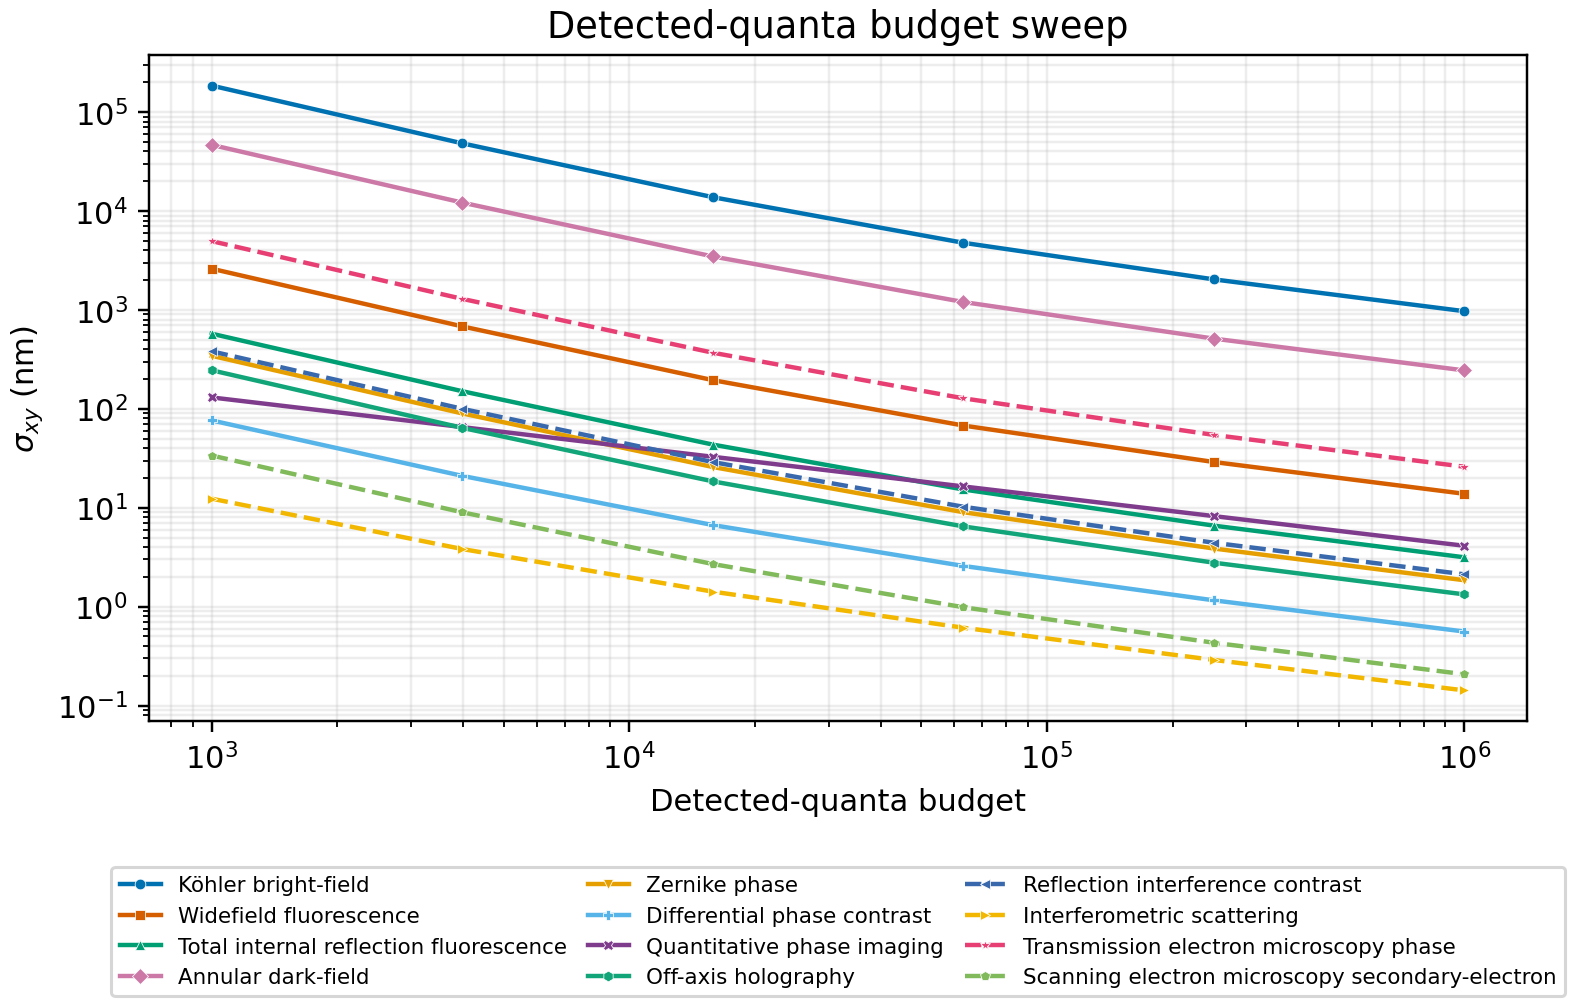
\includegraphics[width=0.85\linewidth]{figures/detected-quanta-budget-pareto.png}
\caption{Detected-quanta-budget sweep for Contract-Q. Each color/marker/line-style combination is one imaging modality, identified by the legend below the axes. Sweeping the plotted budget range within this configured profile shows whether the diagnostic ordering is stable or budget-dependent there. The plotted curves are accompanied by the Contract-Q spectral sampling diagnostics in Table~\ref{tab:detected-quanta-spectral-diagnostics}; singular budget cases are treated as nonfinite rather than assigned artificial finite values.}
\label{fig:detected-quanta-budget-pareto}
\end{figure}
}{%
\generatedfallbackfigure{fig:detected-quanta-budget-pareto}{Detected-quanta-budget sweep. Sweeping the plotted budget range within this configured profile shows whether the ordering is stable or budget-dependent there. Singular budget cases are treated as nonfinite rather than assigned artificial finite values.}{Required figure asset.}
}

\paragraph{Fusion Cram\'{e}r--Rao bound.} Best-$k$ subset search reports the lowest-bound single microscope candidate, the lowest-bound subset at each size, and full-library fusion in \cref{tab:fusion-crlb,fig:fusion-curve}. For these reported curves, Contract-LP is the underlying modality contract unless explicitly stated; each fused subset inherits the spectral lateral sampling/support status of its parent candidates from Table~\ref{tab:lateral-spectral-diagnostics}. The fusion bound is monotonically non-increasing with subset size under independent noise Fisher additivity. A lateral registration covariance can be supplied to model subpixel cross-channel alignment error before summing Fisher matrices; \cref{tab:registration-degradation} reports the corresponding synthetic degradation check. The full-library row is an algebraic independent-channel diagnostic, not a proposed physically simultaneous instrument. In experimental design, users should only fuse candidate microscopes whose physical channels are independently acquired, mutually compatible with the same sample state, and not alternate reconstructions of the same detected quanta.

\IfFileExists{figures/modality-fusion-crlb-table.tex}{%
\begin{table}[H]
\centering
\small
\resizebox{\linewidth}{!}{\begin{tabular}{r p{0.43\linewidth} r r p{0.20\linewidth}}
\toprule
$k$ & Modalities used & Fusion $\sigma_{xy}$ (nm) & Precision gain ($\sigma_{xy}^{(1)}/\sigma_{xy}^{(k)}$) & Interpretation \\
\midrule
1 & Zernike phase contrast & 0.013 & 1.000 & physically\_feasible\_fusion \\
2 & Zernike phase contrast, interferometric scattering microscopy & 0.010 & 1.273 & physically\_feasible\_fusion \\
3 & Zernike phase contrast, off-axis digital holography, interferometric scattering microscopy & 0.010 & 1.311 & physically\_feasible\_fusion \\
4 & Zernike phase contrast, off-axis digital holography, interferometric scattering microscopy, scanning electron microscopy secondary-electron & 9.760e-03 & 1.347 & algebraic\_diagnostic\_only \\
5 & Zernike phase contrast, differential phase contrast, off-axis digital holography, interferometric scattering microscopy, scanning electron microscopy secondary-electron & 9.712e-03 & 1.354 & algebraic\_diagnostic\_only \\
6 & Zernike phase contrast, differential phase contrast, off-axis digital holography, reflection interference contrast microscopy, interferometric scattering microscopy, scanning electron microscopy secondary-electron & 9.692e-03 & 1.357 & algebraic\_diagnostic\_only \\
7 & Zernike phase contrast, differential phase contrast, quantitative phase imaging, off-axis digital holography, reflection interference contrast microscopy, interferometric scattering microscopy, scanning electron microscopy secondary-electron & 9.691e-03 & 1.357 & algebraic\_diagnostic\_only \\
8 & Zernike phase contrast, differential phase contrast, quantitative phase imaging, off-axis digital holography, reflection interference contrast microscopy, interferometric scattering microscopy, transmission electron microscopy phase contrast, scanning electron microscopy secondary-electron & 9.691e-03 & 1.357 & algebraic\_diagnostic\_only \\
9 & partially coherent Köhler bright-field, Zernike phase contrast, differential phase contrast, quantitative phase imaging, off-axis digital holography, reflection interference contrast microscopy, interferometric scattering microscopy, transmission electron microscopy phase contrast, scanning electron microscopy secondary-electron & 9.691e-03 & 1.357 & algebraic\_diagnostic\_only \\
10 & partially coherent Köhler bright-field, annular Köhler dark-field, Zernike phase contrast, differential phase contrast, quantitative phase imaging, off-axis digital holography, reflection interference contrast microscopy, interferometric scattering microscopy, transmission electron microscopy phase contrast, scanning electron microscopy secondary-electron & 9.691e-03 & 1.357 & algebraic\_diagnostic\_only \\
11 & partially coherent Köhler bright-field, widefield fluorescence, annular Köhler dark-field, Zernike phase contrast, differential phase contrast, quantitative phase imaging, off-axis digital holography, reflection interference contrast microscopy, interferometric scattering microscopy, transmission electron microscopy phase contrast, scanning electron microscopy secondary-electron & 9.691e-03 & 1.357 & algebraic\_diagnostic\_only \\
12 & all 12 implemented modalities & 9.691e-03 & 1.357 & algebraic\_diagnostic\_only \\
\bottomrule
\end{tabular}
 and %% Generated by assemble-no-figures script
\endinput
}
\caption{Best-$k$ fusion Cram\'{e}r--Rao bound over the configured microscope candidates. Rows are selected by lowest fused $\sigma_{xy}$ under the algebraic independent-channel search and inherit the Contract-LP spectral sampling/support status of their parent candidates. The fused subsets should not be read as physically simultaneous instrument designs unless the selected channels have independent acquisition budgets, calibrated registration, and sample compatibility.}
\label{tab:fusion-crlb}
\end{table}
}{%
\generatedfallbacktable{tab:fusion-crlb}{Best-$k$ fusion Cram\'{e}r--Rao bound over the configured microscope candidates.}{Required table asset.}
}

\IfFileExists{figures/modality-fusion-crlb.png}{%
\begin{figure}[H]
\centering
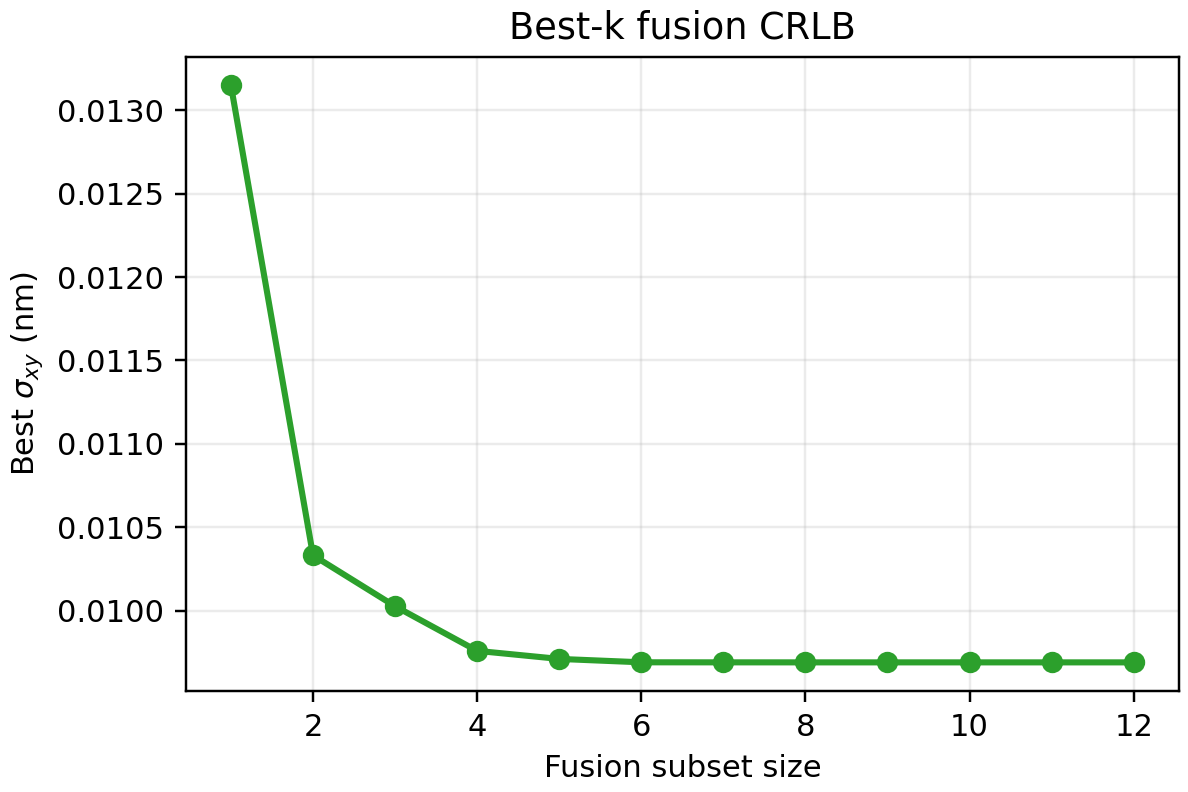
\includegraphics[width=0.85\linewidth]{figures/modality-fusion-crlb.png}
\caption{Fusion Cram\'{e}r--Rao bound versus subset size. Monotonicity follows from independent noise Fisher additivity. Under this profile, most of the lateral information is already captured by the first few selected microscope candidates; the curve inherits the Contract-LP spectral sampling/support status of its selected parent candidates.}
\label{fig:fusion-curve}
\end{figure}
}{%
\generatedfallbackfigure{fig:fusion-curve}{Fusion Cram\'{e}r--Rao bound versus subset size. The lowest attainable lateral bound is non-increasing as independent candidate Fisher matrices are added.}{Required figure asset.}
}

\IfFileExists{figures/fusion-independence-metadata-table.tex}{%
\begin{table}[H]
\centering
\small
\resizebox{\linewidth}{!}{\begin{tabular}{rp{0.36\linewidth}p{0.22\linewidth}p{0.20\linewidth}c}
\toprule
$k$ & Modalities & Physical status & Interpretation & Needs physical design review? \\
\midrule
1 & Zernike phase contrast & physically\_feasible\_sequential\_or\_simultaneous & physically\_feasible\_fusion & no \\
2 & Zernike phase contrast, interfero\allowbreak{}metric scattering microscopy & physically\_feasible\_sequential\_or\_simultaneous & physically\_feasible\_fusion & no \\
3 & Zernike phase contrast, off-axis digital holography, interfero\allowbreak{}metric scattering microscopy & physically\_feasible\_sequential\_or\_simultaneous & physically\_feasible\_fusion & no \\
4 & Zernike phase contrast, off-axis digital holography, interfero\allowbreak{}metric scattering microscopy, scanning electron microscopy secondary-electron & incompatible\_hard\_stop & algebraic\_diagnostic\_only & yes \\
12 & all 12 implemented modalities & incompatible\_hard\_stop & algebraic\_diagnostic\_only & yes \\
\bottomrule
\end{tabular}
}
\caption{Fusion-independence metadata emitted with representative best-$k$ subsets. The last column answers whether the subset still needs physical design review before interpreting the algebraic Fisher sum as an experimental acquisition.}
\label{tab:fusion-independence-metadata}
\end{table}
}{}

The lowest-bound $k$-subset curve saturates after the selected microscope candidates under this diagnostic profile because the leading scanning-electron, off-axis-holography, and interferometric-scattering terms already account for most of the lateral Fisher contribution in the configured profiles. The flat tail is profile-specific; it does not imply that large candidate libraries are generally redundant.

This serial-allocation solution is a boundary solution under fixed per-frame equal costs and the configured profiles; it inherits the Contract-LP spectral sampling/support status of the parent rows in Table~\ref{tab:lateral-spectral-diagnostics}. It should not be interpreted as a recommendation to replace optical live-particle workflows with SEM or other modalities, because practical compatibility, vacuum, dose, sample preparation, and field-of-view constraints are outside this synthetic objective model.

\IfFileExists{figures/time-allocation-crlb-table.tex}{%
\begin{table}[H]
\centering
\small
\resizebox{\linewidth}{!}{\begin{tabular}{l p{0.30\linewidth} r r r p{0.14\linewidth} p{0.16\linewidth}}
\toprule
Criterion & Nonzero allocation & $\sigma_{xy}$ (nm) & Gain vs. uniform & Gain vs. best single & Status & Termination \\
\midrule
A & zernike\_phase\_contrast:1 & 0.013 & 6.519 & 1.000 & invalid & no\_descent\_direction \\
D & zernike\_phase\_contrast:1 & 0.013 & 42.50 & 1.000 & invalid & no\_descent\_direction \\
E & zernike\_phase\_contrast:1 & 0.013 & 6.572 & 1.000 & invalid & no\_descent\_direction \\
\bottomrule
\end{tabular}
}
\caption{Serial time-allocation Cram\'{e}r--Rao diagnostic over the configured microscopes. Each row solves the fixed-time allocation problem for the stated A-, D-, or E-optimal scalarization using the same per-microscope Fisher matrices as the lateral Contract-LP diagnostic and therefore inherits their spectral sampling/support status. The allocation column reports nonzero time fractions under a unit total-time budget and equal per-frame time costs.}
\label{tab:time-allocation-crlb}
\end{table}
}{}

\IfFileExists{figures/registration-degradation-table.tex}{%
\begin{table}[H]
\centering
\small
\resizebox{\linewidth}{!}{\begin{tabular}{r r r r}
\toprule
Registration covariance diagonal (diagnostic coordinate units$^2$) & Fusion $\sigma_{xy}$ (nm) & Fusion gain & Degradation \\
\midrule
$0.00$ & $0.671$ & $1.139$ & $0.0\%$ \\
$0.01$ & $0.680$ & $1.122$ & $1.4\%$ \\
$0.10$ & $0.759$ & $1.006$ & $13.2\%$ \\
\bottomrule
\end{tabular}
}
\caption{Registration-covariance degradation diagnostic. Increasing residual cross-channel alignment covariance monotonically weakens the fused bound for the named modality subset. The diagnostic inherits the Contract-LP spectral sampling/support status of the fused modalities; the covariance entries are in nm$^2$ on the shared lateral $x/y$ parameter block.}
\label{tab:registration-degradation}
\end{table}
}{}

\paragraph{Per-pixel Fisher density.} The Cram\'{e}r--Rao implementation computes the per-pixel Fisher information integrand rather than only its spatial sum. The maps in \cref{fig:fisher-density-panel} localize the detector pixels with high Fisher contribution for the plotted modality profiles and can serve as optional information-aware training targets when a downstream model is configured for that auxiliary target.

\IfFileExists{figures/fisher-density-panel.png}{%
\begin{figure}[H]
\centering
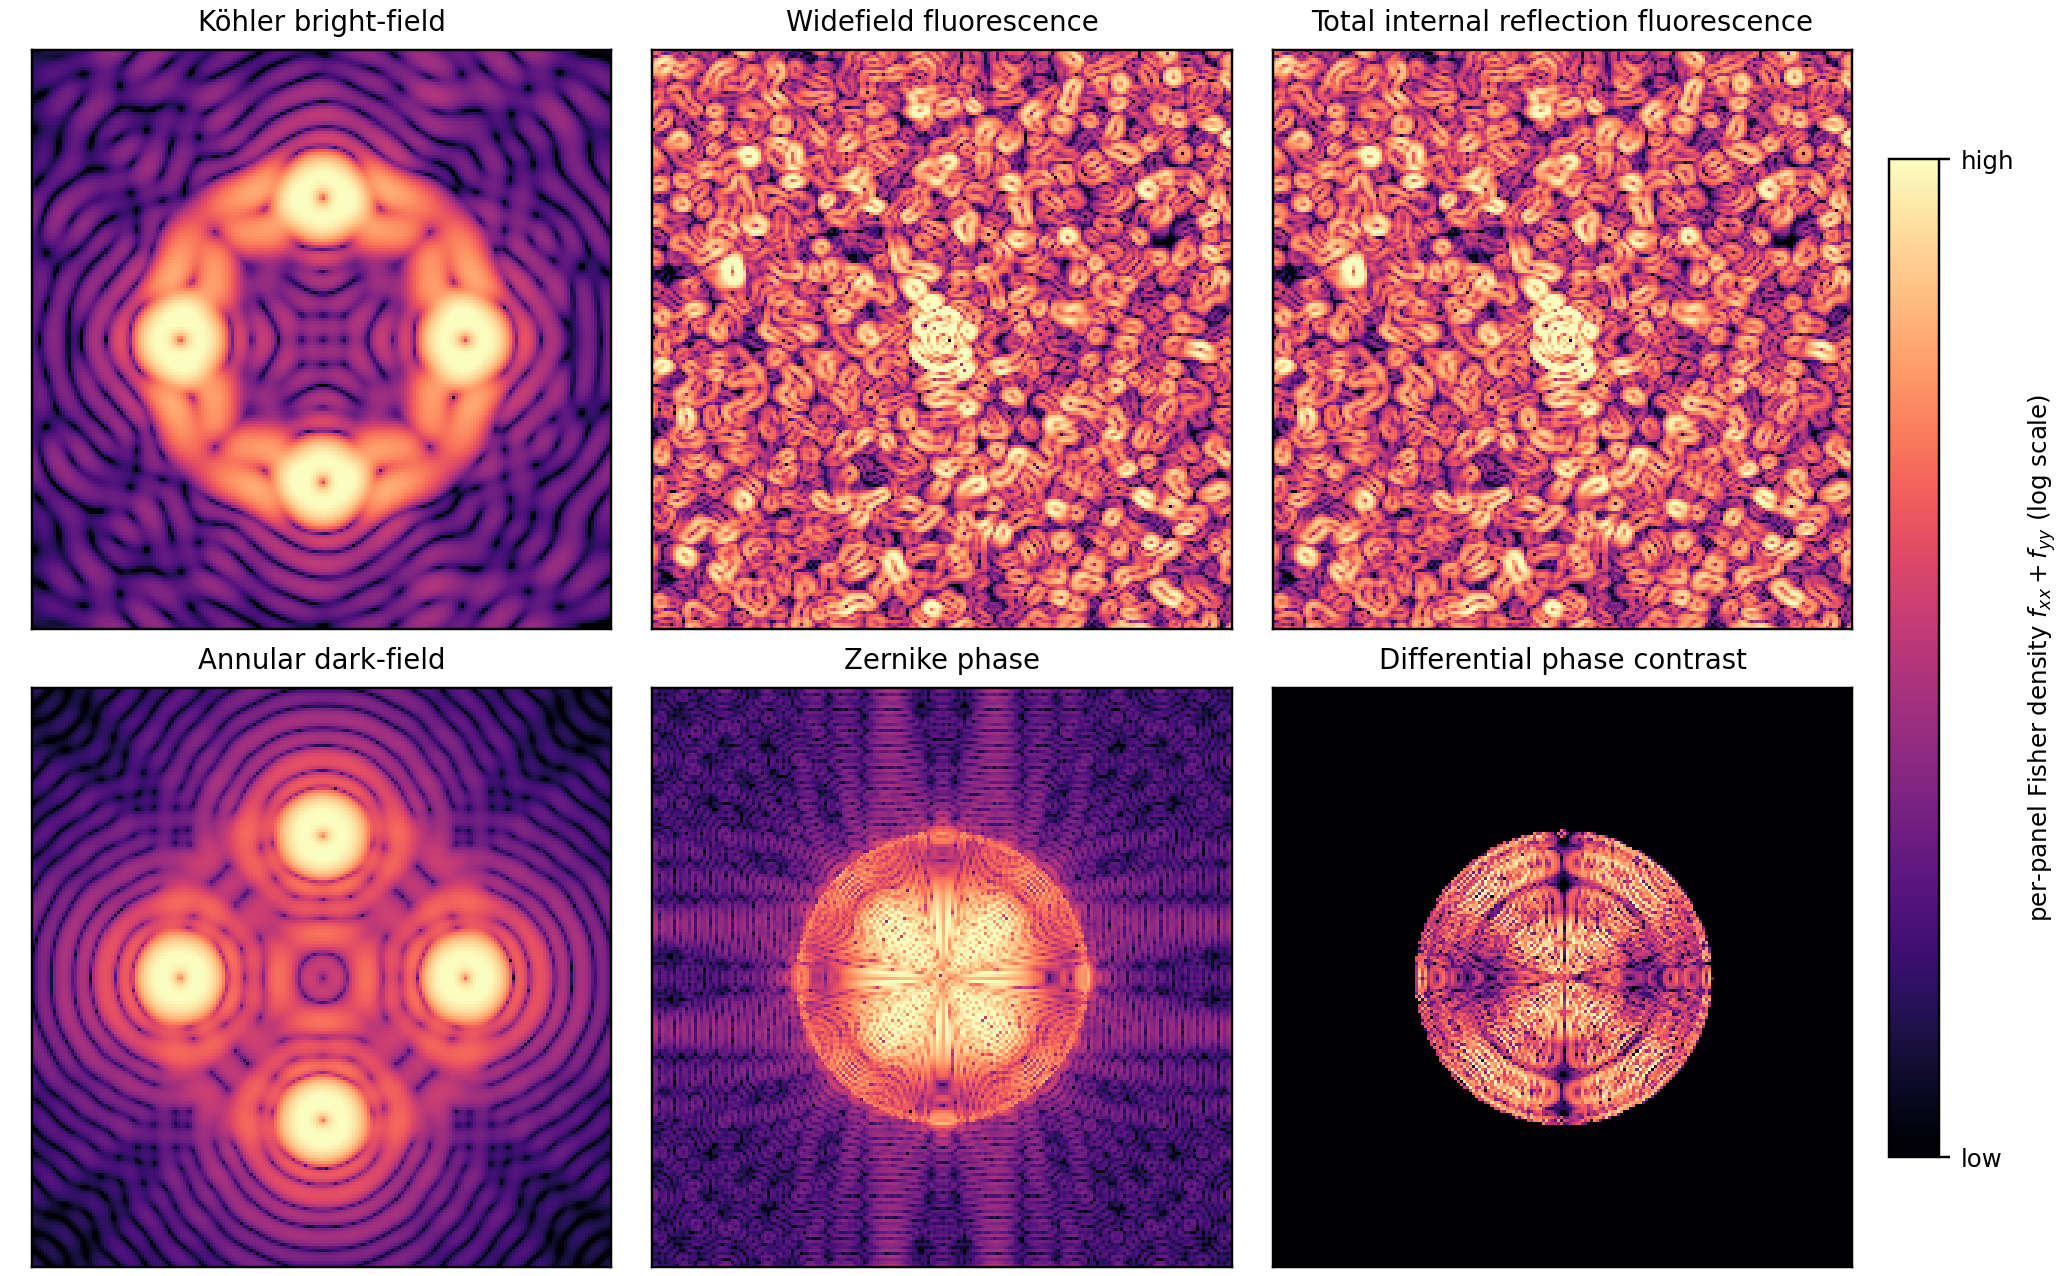
\includegraphics[width=\linewidth]{figures/fisher-density-panel.png}
\caption{Per-pixel Fisher information density maps. Each panel visualizes $f_{xx}+f_{yy}$ for one modality profile on the same particle. Each panel is independently log-scaled and percentile-clipped; the magma colorbar runs from dark (low) to bright (high) per-pixel Fisher density, and carries only that direction rather than a shared absolute scale.}
\label{fig:fisher-density-panel}
\end{figure}
}{%
\generatedfallbackfigure{fig:fisher-density-panel}{Per-pixel Fisher information density maps. Each panel visualizes $f_{xx}+f_{yy}$ for one modality profile on the same particle.}{Required figure asset.}
}

\paragraph{Implementation consistency diagnostics.} The following deterministic diagnostics are software consistency checks for the implemented Fisher and supervision layers. They verify expected algebraic behavior under controlled synthetic inputs; they are not empirical validation of microscope performance.

\Cref{tab:loewner-dominance} isolates the fixed-budget Loewner-dominance diagnostic with a two-matrix synthetic example.

\IfFileExists{figures/loewner-dominance-summary-table.tex}{%
\begin{table}[H]
\centering
\small
\resizebox{\linewidth}{!}{\begin{tabular}{p{0.20\linewidth}p{0.28\linewidth}p{0.16\linewidth}p{0.28\linewidth}}
\toprule
Pair & Information-rate test & Min. eigenvalue & Allocation effect \\
\midrule
A vs. B & $A_{A}-A_{B}\succeq 0$ & $2.0$ & keep A \\
B vs. A & $A_{B}-A_{A}\not\succeq 0$ & $-3.0$ & prune B if no minimum allocation is required \\
\bottomrule
\end{tabular}
}
\caption{Fixed-budget scheduling diagnostic. The table is a synthetic two-matrix check illustrating Loewner dominance, not a pair of real microscope modalities.}
\label{tab:loewner-dominance}
\end{table}
}{}

\Cref{tab:structured-background-loss} reports the structured-background nuisance projection diagnostic used to check that signed derivative maps, rather than squared information-density maps, are used for Schur-complement information loss.

\IfFileExists{figures/structured-background-loss-table.tex}{%
\begin{table}[H]
\centering
\small
\begin{tabular}{lccc}
\toprule
Diagnostic state & $F_{xx}$ & $F_{yy}$ & Mean loss over $x,y$ \\
\midrule
Raw particle derivatives & $50.0$ & $50.0$ & -- \\
After linear-$x$ nuisance projection & $0.0$ & $50.0$ & $50\%$ \\
\bottomrule
\end{tabular}

\caption{Structured-background nuisance projection diagnostic. The output is computed from signed lateral derivative maps for the named modality profile, noise-weighted inner products, and Schur-complement projection against the listed nuisance basis maps.}
\label{tab:structured-background-loss}
\end{table}
}{}

\subsection{Measurement-supported supervision}

The supervision consistency evaluation in \cref{tab:supervision-audit} evaluates deterministic particle-frame cases spanning supported, borderline, and singular zero-contrast targets without depending on Segment Anything Model 2. This deterministic evaluation set is not a population estimate for the full training corpus; it tests whether positive object pixels remain supervised while unsupported known-object pixels are routed to the ignore mask rather than silently converted to background.

\IfFileExists{figures/supervision-audit-table.tex}{%
\begin{table}[H]
\centering
\small
\begin{tabular}{p{0.40\linewidth}p{0.22\linewidth}p{0.28\linewidth}}
\toprule
Metric & Value & Check \\
\midrule
Particle-frame cases & 3 & deterministic evaluation set \\
Positive supervision pixel fraction & 33.3\% & supported target supervised \\
Ignored known-object pixels & 66.7\% & unsupported pixels ignored \\
Ignored particle fraction & 66.7\% & object-level support gate \\
Low-signal particle fraction & 66.7\% & signal factor \\
High-bound particle fraction & 66.7\% & information factor \\
Fisher-singular fraction & 33.3\% & singular-bound handling \\
Supported records & 1 & supported-case count \\

\end{tabular}
\caption{Supervision-schema consistency evaluation on a deterministic particle-frame set. Count rows are integers; support and exclusion rows are fractions of the deterministic evaluation set.}
\label{tab:supervision-audit}
\end{table}
}{%
\generatedfallbacktable{tab:supervision-audit}{Supervision-schema consistency evaluation on a deterministic particle-frame set.}{Required table asset.}
}

The deterministic supervision audit is the paper-facing supervision result. It verifies the simulator-side mask contract without promoting any downstream model-training run, checkpoint, or real-video transfer example to manuscript evidence.
